%%==================================================
%% thesis.tex
%%==================================================

% 双面打印
%\documentclass[doctor, adobefonts, openright, twoside, cs4size]{sjtuthesis}
 \documentclass[bachelor, winfonts, openany, oneside, cs4size, review]{sjtuthesis} 
% \documentclass[master, adobefonts, review]{sjtuthesis} 
% \documentclass[%
%   bachelor|master|doctor,	% 必选项
%   adobefonts|winfonts,  	% 只测试了adobefonts,请使用adobefonts
%   oneside|twoside,		% 单面打印,双面打印(奇偶页交换页边距,默认)
%   openany|openright, 		% 可以在奇数或者偶数页开新章|只在奇数页开新章(默认)
%   cs4size|c5size, 		% 正文字号:小四、五号(默认)
%   review,	 		% 盲审论文,隐去作者姓名、学号、导师姓名、致谢、发表论文和参与的项目
%   submit			% 定稿提交的论文,插入签名扫描版的原创性声明、授权声明 
% ]

% 逐个导入参考文献数据库
\addbibresource{bib/thesis.bib}
% \addbibresource{bib/chap2.bib}

\begin{document}

%% 无编号内容:中英文论文封面、授权页
\title{上海交通大学学位论文 \LaTeX 模板示例文档}
\author{某\quad{}某}
\advisor{某某教授}
% \coadvisor{某某教授}
\defenddate{2014年12月17日}
\school{上海交通大学}
\institute{某某系}
\studentnumber{0010900990}
\major{某某专业}

\englishtitle{A Sample Document for \LaTeX-basedd SJTU Thesis Template}
\englishauthor{\textsc{Mo Mo}}
\englishadvisor{Prof. \textsc{Mou Mou}}
% \englishcoadvisor{Prof. \textsc{Uom Uom}}
\englishschool{Shanghai Jiao Tong University}
\englishinstitute{\textsc{Depart of XXX, School of XXX} \\
  \textsc{Shanghai Jiao Tong University} \\
  \textsc{Shanghai, P.R.China}}
\englishmajor{A Very Important Major}
\englishdate{Dec. 17th, 2014}


%\maketitle
\newMaketitle

%\makeenglishtitle
%\newMakeenglishtitle

\makeatletter
\ifsjtu@submit\relax
	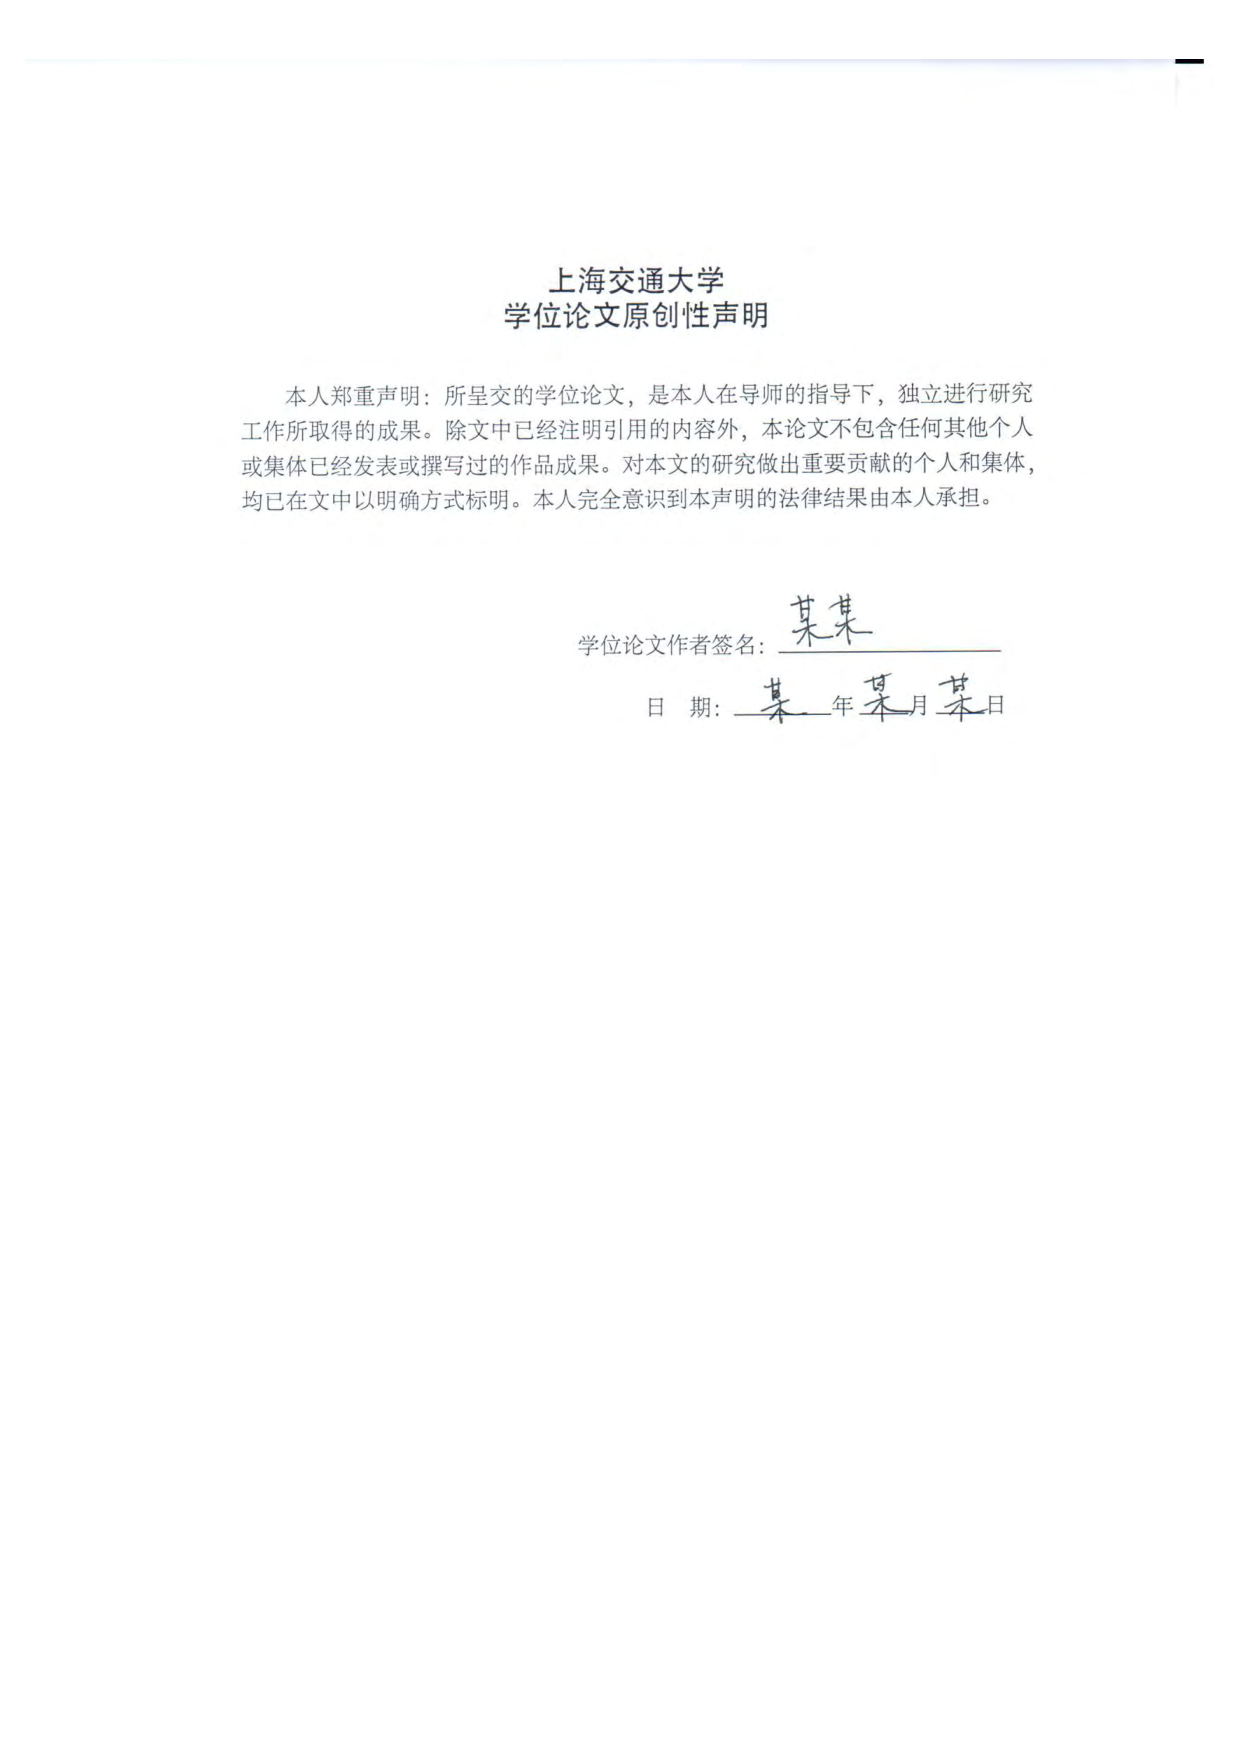
\includepdf{pdf/original.pdf}
	\cleardoublepage
	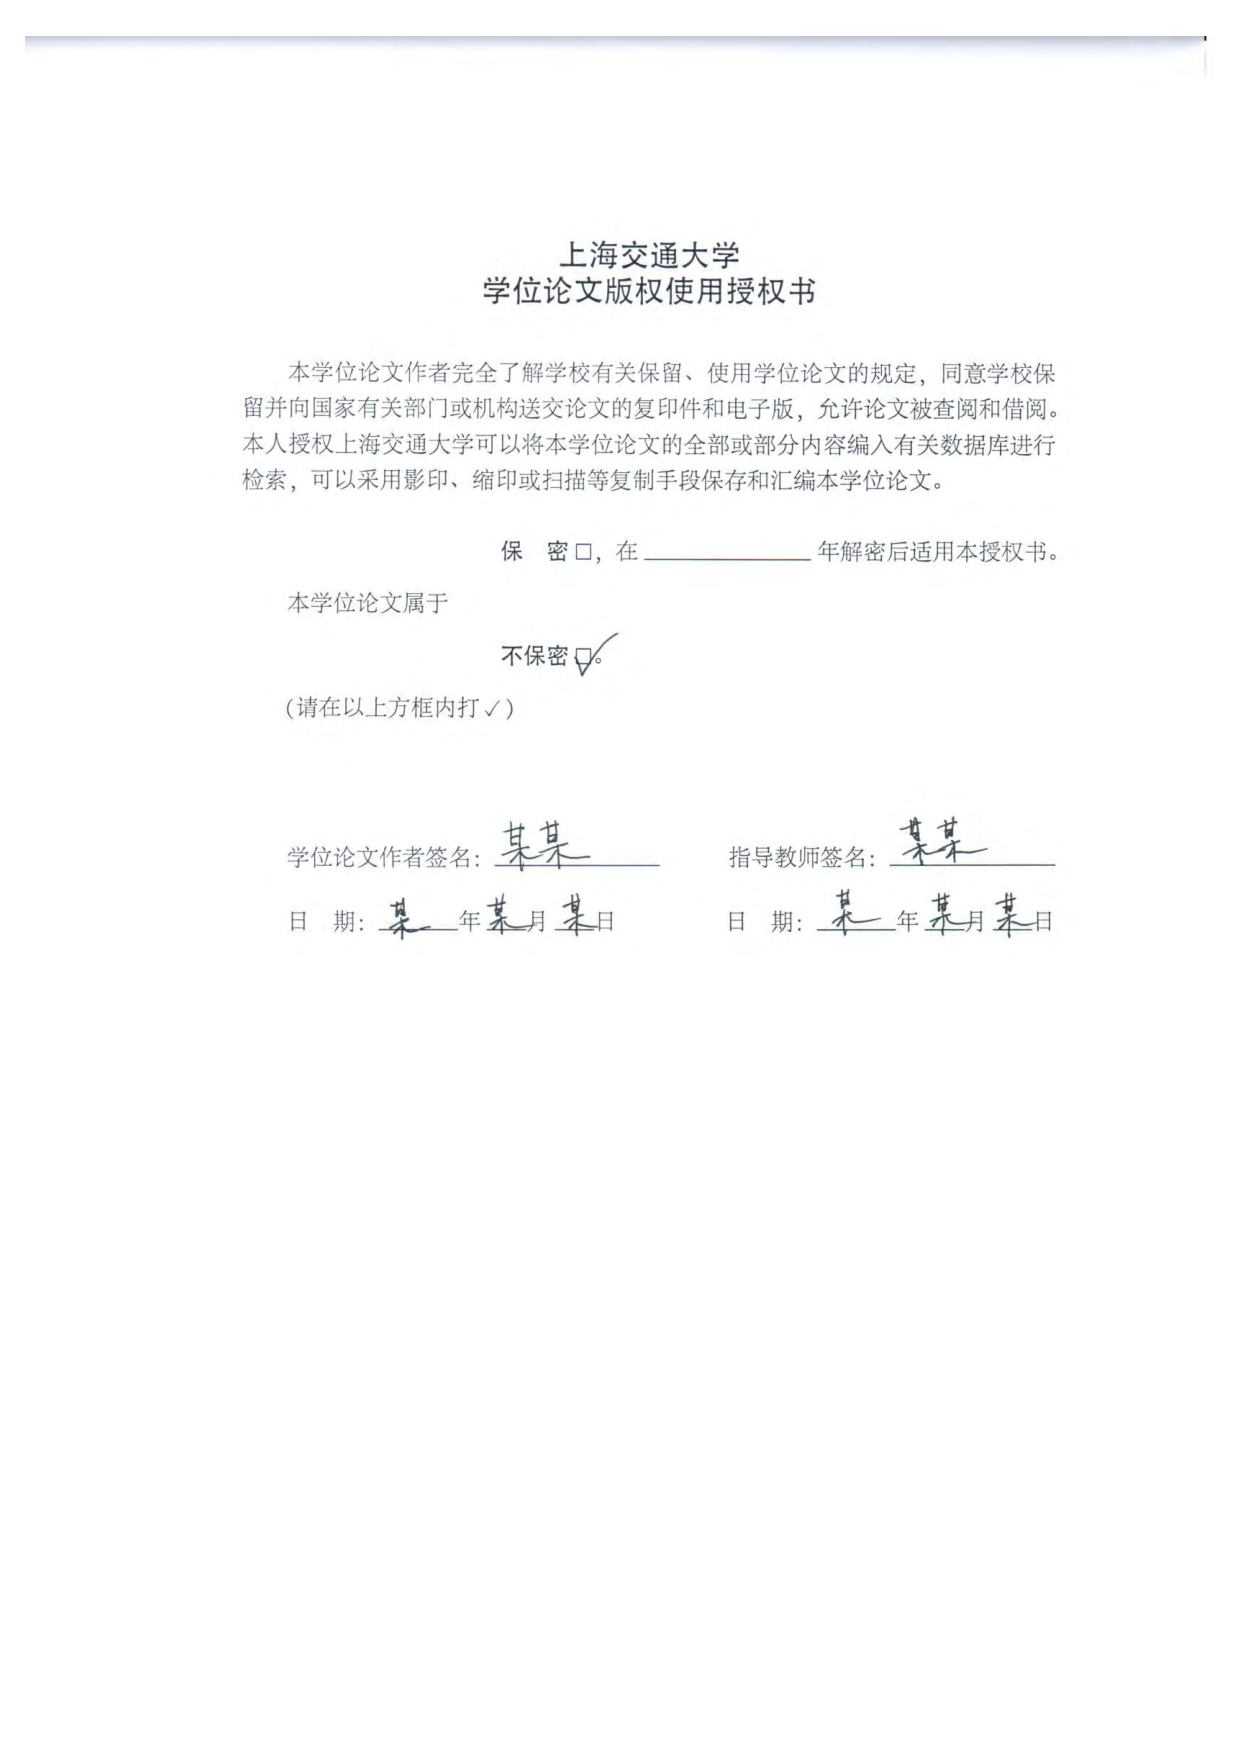
\includepdf{pdf/authorization.pdf}
	\cleardoublepage
\else
	%\makeDeclareOriginal
	%\makeDeclareAuthorization
\fi
\makeatother


\frontmatter 	% 使用罗马数字对前言编号

%% 摘要
\pagestyle{main}
%%==================================================
%% abstract.tex for SJTU Master Thesis
%%==================================================

\begin{abstract}

随着社会的信息化,地球已成为地球村,人与人之间的距离缩短、联系更加紧密。而现在,物联网作为一种新的网络模式,也渐渐进入人们的实现,并越来越得到重视。从宏观上讲,我国已经把发展研究物联网作为战略上的要求;从微观上讲,现在市场上开始出现的一些智能家居,以及现在的车联网都是物联网的一种体现。虽然物联网现在的发展和研究都仍处于起步阶段,对于物联网的各种标准都尚未有明确规定,导致各厂商之间都是按照自己的标准行事,使得物联网这个产业其实一定程度上很混乱。然而不论日后对于物联网会有什么标准,必然都会包含安全这一方面的标准。由于互联网的各种安全事件的发生,我们已经见识到安全是多么的重要,因此在物联网这种与生活更紧密结合的模式中必定对于安全有更严格的要求。而Trivium则可能是适应未来物联网时代的一种算法。
Trivium算法作为一种基于硬件的流密码算法,是欧洲流密码工程eSTREAM的最终胜选算法之一,由Christophe De Canniere和Bart Preneel提出,在其出现之后就有在密码界引起了关注,因为其设计简单优美,而且也宣传它具有很强的安全性,因此只要其安全性得到验证,就十分适合用来作为物联网中的密码算法。

\keywords{\large Trivium \quad 物联网 \quad 流密码}
\end{abstract}

\begin{englishabstract}



\englishkeywords{\large Trivium, Internet of Things, stream ciphers}
\end{englishabstract}



%% 目录、插图目录、表格目录
\tableofcontents
% \listoffigures
% \addcontentsline{toc}{chapter}{\listfigurename} %将插图目录加入全文目录
% \listoftables
% \addcontentsline{toc}{chapter}{\listtablename}  %将表格目录加入全文目录
% \listofalgorithms
% \addcontentsline{toc}{chapter}{代码索引}  %将表格目录加入全文目录

% %%==================================================
%% symbol.tex for SJTUThesis
%% Encoding: UTF-8
%%==================================================

\chapter{主要符号对照表}
\label{chap:symb}

\begin{longtable}{rl}
$\epsilon$     & 介电常数 \\
 $\mu$ 		& 磁导率 \\
 $\epsilon$     & 介电常数 \\
 $\mu$ 		& 磁导率 \\
 $\epsilon$     & 介电常数 \\
 $\mu$ 		& 磁导率 \\
 $\epsilon$ 	& 介电常数 \\
 $\mu$ 		& 磁导率 \\
 $\epsilon$     & 介电常数 \\
 $\mu$ 		& 磁导率 \\
 $\epsilon$     & 介电常数 \\
 $\mu$ 		& 磁导率 \\
 $\epsilon$     & 介电常数 \\
 $\mu$ 		& 磁导率 \\
 $\epsilon$ 	& 介电常数 \\
 $\mu$ 		& 磁导率 \\
 $\epsilon$     & 介电常数 \\
 $\mu$ 		& 磁导率 \\
 $\epsilon$     & 介电常数 \\
 $\mu$ 		& 磁导率 \\
 $\epsilon$     & 介电常数 \\
 $\mu$ 		& 磁导率 \\
 $\epsilon$ 	& 介电常数 \\
 $\mu$ 		& 磁导率 \\
 $\epsilon$     & 介电常数 \\
 $\mu$ 		& 磁导率 \\
 $\epsilon$     & 介电常数 \\
 $\mu$ 		& 磁导率 \\
 $\epsilon$     & 介电常数 \\
 $\mu$ 		& 磁导率 \\
 $\epsilon$ 	& 介电常数 \\
 $\mu$ 		& 磁导率 \\
 $\epsilon$     & 介电常数 \\
 $\mu$ 		& 磁导率 \\
 $\epsilon$     & 介电常数 \\
 $\mu$ 		& 磁导率 \\
 $\epsilon$     & 介电常数 \\
 $\mu$ 		& 磁导率 \\
 $\epsilon$ 	& 介电常数 \\
 $\mu$ 		& 磁导率 \\
 $\epsilon$     & 介电常数 \\
 $\mu$ 		& 磁导率 \\
 $\epsilon$     & 介电常数 \\
 $\mu$ 		& 磁导率 \\
 $\epsilon$     & 介电常数 \\
 $\mu$ 		& 磁导率 \\
 $\epsilon$ 	& 介电常数 \\
 $\mu$ 		& 磁导率 \\
 $\epsilon$     & 介电常数 \\
 $\mu$ 		& 磁导率 \\
 $\epsilon$     & 介电常数 \\
 $\mu$ 		& 磁导率 \\
 $\epsilon$     & 介电常数 \\
 $\mu$ 		& 磁导率 \\
\end{longtable}
 % 主要符号、缩略词对照表

\mainmatter	% 使用阿拉伯数字对正文编号

%% 正文内容
\pagestyle{main}
%%==================================================
%% chapter01.tex for SJTU Master Thesis
%%==================================================

\chapter{绪论}
\label{chap:introduction}

\section{Trivium算法的简单介绍}

Trivium算法是一种基于硬件的流密码算法,是欧洲流密码工程eSTREAM的最终胜选算法之一。其设计初衷是想试验是否存在一种简单的流密码算法能够兼具高效性、可变性以及最重要的安全性。

由于物联网中各种芯片的逻辑门数肯定会有所限制,因此可能无法实现复杂的加密算法,所以作为流密码的Trivium似乎是一种不错的选择。因此Trivium算法的安全性和效率直接关系到未来的物联网中是否能使用Trivium算法作为一种加密标准被广泛采用。因此本文将对Trivium的安全性和效率进行研究。

通过对Trivium算法的安全性和效率的研究,本文著者希望给出在物联网中Trivium算法是否是合适的加密算法的判断,并且对Trivium算法加以改进,以使其更适合物联网的使用环境。

具体地,本文研究了Trivium算法以及具有与Trivium算法相似结构的Trivium型算法,计算了Trivium型算法的内部状态位数的下限,并构造了几种能产生小周期的初始内部状态,通过分析构造方法,分析Trivium算法及Trivium型算法中的具体使用步骤是否安全。


\section{物联网发展与现状}

物联网这一概念出现至今已超过10年时间,然而仍然没有一个统一且明确的定义。

1999年,MITAutoIDCenter给出了早期的“物联网”定义:在计算机互联网的基础上,利用RFID、无线数据通信等技术,构造一个覆盖世界上各种事物的网络(InternetofThings),以实现自动识别物品和互联共享信息\parencite{宁焕生2010全球物联网发展及中国物联网建设若干思考}。

2005年,国际电信联盟(ITU)发布的《ITU互联网报告2005:物联网》中正式给出了“物联网”概念并对扩展了其涵义,指出物联网是互联网应用的延伸,实现物联网的四大核心技术将是“RFID、传感器技术、纳米技术、智能嵌入技术”\parencite{宁焕生2010全球物联网发展及中国物联网建设若干思考}。

2009年9月,欧盟公布的一份CERPIoTSRA中,将“物联网”定义为:物联网将是未来互联网不可分割的一部分,是一个动态的全球网络架构,它具备基于一定的标准和互用的通信协议的自组织能力.其中物理的和虚拟的“物”均具有身份标识、物理属性和虚拟特性,并应用智能接口可以无缝链接到信息网络\parencite{宁焕生2010全球物联网发展及中国物联网建设若干思考}。

自2009年IBM提出“智慧地球”这一概念后,物联网在全球掀起了一股浪潮,美国、欧洲、我国都把物联网作为战略发展计划。然而物联网的发展却仍只是停留在起步阶段,且不论上述的对于物联网这一概念都尚未有明确统一的定义,对于物联网中要用的标识码、各种标准各国之间哪怕是一个国家内的不同厂商也尚未达成一致,因此要有一个严格明确的物联网实际应用实验环境还早的很。现在市场上的物联网相关产品多数是车联网或者智能家居或者物流方面的相关应用,然而这距离物物相连、自动化处理仍很遥远,可以说物联网的现状仍然是处于制定标准阶段以及一些小范围的实验性产品。

\section{本文的研究意义和研究成果}

Trivium算法作为一种新的算法,虽然得到了密码界的大量关注,但发表的对于Trivium算法的相关研究却并不多,其中更是几乎都是对于Trivium算法的攻击研究,而鲜有对Trivium算法的实际应用做研究探讨的。

另外现在的物联网的研究很多都集中在研究分析物联网的发展方向或者体系结构,又或者是将各种现有系统套上物联网,然后研究是否可行或者有什么优劣,却鲜有研究物联网下的安全问题的,因此研究物联网下的密码算法是一项有意义的工作。另外现在的各种加密手段很多都是用RSA、AES、3DES这种,在互联网中,考虑到设备的计算能力,这些都可以接受,但是在物联网时代,是否所有物联网设备都支持就不得而知了,因此研究物联网下的轻量级密码算法Trivium算法是有意义的。

本文的创新工作在于计算了与Trivium算法相似结构的Trivium型算法的内部状态位数的下限,另外给出了构造能产生小周期的初始内部状态的方法。以及提出了将Trivium算法应用到物联网场景下的设计想法。

%%==================================================
%% chapter02.tex for SJTU Master Thesis
%% Encoding: UTF-8
%%==================================================

\chapter{Trivium流密码算法}

\section{标准的Trivium流密码算法}

由Christophe De 和 Bart Preneel设计的标准Trivium算法共有288个内部状态位,这288位内部状态的每一次更新构成了Trivium算法生成密钥流中一位密钥的生成来源, Trivium算法的具体应用步骤如下:

\begin{enumerate}[noitemsep,topsep=0pt,parsep=0pt,partopsep=0pt]
  \item 密钥分配阶段:用户通过事先定义或者协商得到密钥K和初始向量IV。
  \item 初始化阶段:将密钥K和初始向量IV装填入Trivium的288位的内部状态中,并运行几轮Trivium算法更新内部状态。
  \item 密钥流生成阶段:每运行一轮Trivium,更新内部状态并生成一位密钥输出。
\end{enumerate}

下面对每个阶段的具体步骤进行详细描述。

\subsection{Trivium算法内部状态的初始化}

Trivium算法内部状态的初始化,可以用以下步骤描述:

\begin{enumerate}[noitemsep,topsep=0pt,parsep=0pt,partopsep=0pt]
  \item 将Trivium的内部状态分为3个部分,第一部位为1到93位,第二部分为94到177位,第三部分为178到288位。
  \item 将80比特的密钥装填入第一部分的前80位即1到80位,并将第一部分的其他位置0,即81到93位置0。
  \item 将80比特的初始向量装填入第二部分的前80位即94到173位,并将第二部分的其他位置0,即174到177位置0。
  \item 将第三部分的后3位置1,即286到288位置1,并将第三部分的其他位置0,即178到285位置0。
  \item 运行 4*288=1152 轮Trivium算法更新内部状态。
\end{enumerate}

可以使用伪代码算法\ref{algo:trivium_intialize}表示这个过程:

\begin{algorithm}[H]
\caption{Trivium算法内部状态初始化过程}
\label{algo:trivium_intialize}
\begin{algorithmic}

  \STATE {$(S_{1}, S_{2},\ldots, S_{93}) \leftarrow (K_{1}, K_{2}, \ldots, K_{80}, 0, \ldots, 0)$}
  \STATE {$(S_{94}, S_{2},\ldots, S_{177}) \leftarrow (IV_{1}, IV_{2}, \ldots, IV_{80}, 0, \ldots, 0)$}
  \STATE {$(S_{178}, S_{2},\ldots, S_{288}) \leftarrow (0, \ldots, 0, 1, 1, 1)$}
  \FOR {$i \leftarrow 1$ \TO $1152$}
    \STATE {$T_{1} \leftarrow S_{66} + S_{93} + S_{91} * S_{92} + S_{171}$}
    \STATE {$T_{2} \leftarrow S_{162} + S_{177} + S_{175} * S_{174} + S_{264}$}
    \STATE {$T_{3} \leftarrow S_{243} + S_{288} + S_{286} * S_{287} + S_{69}$}
    \FOR {$j \leftarrow 2 $\TO $288$}
     \STATE {$S_{j} \leftarrow S_{j-1}$}
    \ENDFOR
    \STATE {$S_{1} \leftarrow T_{3}$}
    \STATE {$S_{94} \leftarrow T_{1}$}
    \STATE {$S_{178} \leftarrow T_{2}$}
  \ENDFOR

\end{algorithmic}
\end{algorithm}



\subsection{Trivium算法密钥流的生成}
Trivium算法的密钥流生成的过程与Trivium算法的初始化过程基本是完全一致的,唯一的区别在于除了要更新Trivium的内部状态之外,每轮还需要使用6位内部状态位来生成密钥比特。

可以使用伪代码算法\ref{algo:trivium_generate}表示这个过程:

\begin{algorithm}[H]
\caption{Trivium算法密钥流的生成过程}
\label{algo:trivium_generate}
\begin{algorithmic}
  \FOR {$i \leftarrow 1$ \TO $N$}
    \STATE {$R_{1} \leftarrow S_{66} + S_{93}$}
    \STATE {$R_{2} \leftarrow S_{162} + S_{177}$}
    \STATE {$R_{3} \leftarrow S_{243} + S_{288}$}
    \STATE {$Z \leftarrow R_{1} + R_{2} + R_{3}$}
    \STATE {$T_{1} \leftarrow R_{1} + S_{91} * S_{92} + S_{171}$}
    \STATE {$T_{2} \leftarrow R_{2} + S_{175} * S_{174} + S_{264}$}
    \STATE {$T_{3} \leftarrow R_{3} + S_{286} * S_{287} + S_{69}$}
    \FOR {$j \leftarrow 2 $\TO $288$}
     \STATE {$S_{j} \leftarrow S_{j-1}$}
    \ENDFOR
    \STATE {$S_{1} \leftarrow T_{3}$}
    \STATE {$S_{94} \leftarrow T_{1}$}
    \STATE {$S_{178} \leftarrow T_{2}$}
  \ENDFOR
\end{algorithmic}
\end{algorithm}


\subsection{Trivium算法的硬件实现}

\begin{figure}[H]
	\centering
	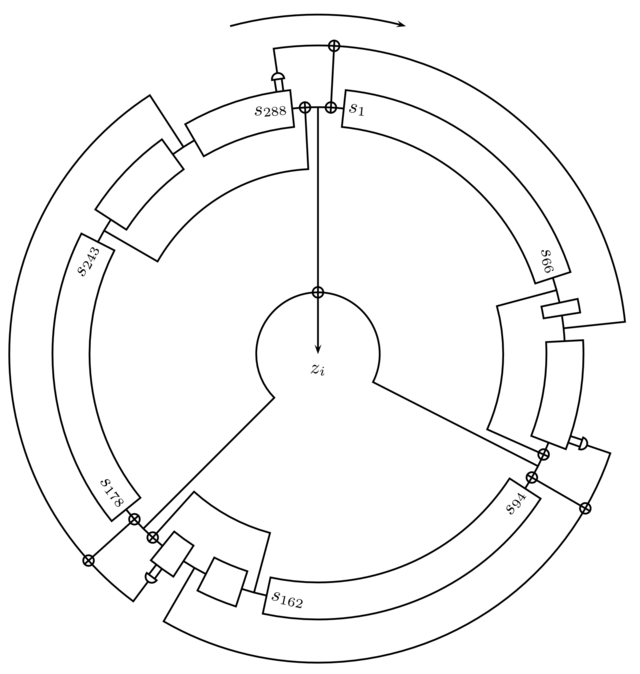
\includegraphics[width=0.5\textwidth]{chap2/hardwareTrivium.png}
	\caption{Trivium算法的硬件实现}\label{fig:Trivium算法的硬件实现}
\end{figure}

\section{Trivium算法的结构}

传统的流密码算法仅有线性反馈移位寄存器实现,因此传统的流密码算法都可以将其表示为一个状态转移矩阵的形式,即存在状态转移矩阵A使$(s_{1}, s_{2}, \ldots, s_{n})^{T}$ = $A_{n*n}$ * $(s_{1}, s_{2}, \ldots, s_{n})^{T}$,然后将状态转移矩阵转化为一个特征多项式进行研究,而Trivium算法除了传统的线性反馈移位寄存器外,还含有三个非线性反馈移位寄存器,因此很难找到一个简单合适的方法将其表示成一个状态转移矩阵或者特征多项式,为了研究方便,本节将先从Trivium算法的线性部分研究Trivium算法的线性部分的结构。

\subsection{Trivium算法的线性部分的状态转移矩阵}

对于仅基于线性反馈移位寄存器的流密码,将其表述成一个状态转移矩阵是一件简单的事,并且通过状态转移矩阵或通过状态转移矩阵得到的特征多项式可以有效地分析密码的性质。虽然Trivium算法包含非线性反馈移位寄存器的部分,但在算法\ref{algo:trivium_intialize}中可以发现$S_{66} + S_{93} + S_{91} * S_{92} + S_{171}$、$S_{162} + S_{177} + S_{175} * S_{174} + S_{264}$、$S_{243} + S_{288} + S_{286} * S_{287} + S_{69}$是Trivium算法中的主要部分,且可以拆成线性部分和非线性部分的组合,形成如$(s_{1}, s_{2}, \ldots, s_{n})^{T}$ = $A_{n*n}$ * $(s_{1}, s_{2}, \ldots, s_{n})^{T}$ + $(w_{1}, w_{2}, \ldots, w_{n})^{T}$的形式。

对于Trivium算法的线性部分,我们可以得到如下方程:

令
\begin{align}
\label{eq:struct_A}
& A = \left(
\begin{array}{@{}*{6}{c}@{}}
0 & 0 & 0 & \cdots & 0 & 1 \\
1 & 0 & 0 & \cdots & 0 & 0 \\
0 & 1 & 0 & \cdots & 0 & 0 \\
\vdots & & \ddots & & & \vdots \\
\vdots & & & \ddots & & \vdots \\
0 & 0 & 0 & \cdots & 1 & 0 \\
\end{array}
\right)+\left(
\begin{array}{@{}*{9}{c}@{}}
0 & \cdots & 1_{(1,69)} & \cdots & 0 & \cdots & 1_{(1,243)} & \cdots & 0 \\
0 & \cdots & \cdots & \cdots & 0 & \cdots & \cdots & \cdots & 0 \\
\vdots & & & & & & & & \vdots \\
0 & \cdots & 1_{(94,66)} & \cdots & 0 & \cdots & 1_{(94,171)} & \cdots & 0 \\
\vdots & & & & & & & & \vdots \\
0 & \cdots & \cdots & 1_{(178,162)}  & \cdots & \cdots & 1_{(178,264)} & \cdots & 0 \\
\vdots & & & & & & & & \vdots \\
0 & \cdots & \cdots & \cdots & 0 & \cdots & \cdots & \cdots & 0 \\
\end{array}
\right)
\end{align}

\begin{align}
\label{eq:struct_S}
& S = \left(
\begin{array}{@{}*{6}{c}@{}}
S_{1} \\
S_{2} \\
\vdots \\
S_{288} \\
\end{array}
\right)
\end{align}

\begin{align}
\label{eq:struct_C}
& C = \left(
\begin{array}{@{}*{6}{c}@{}}
S_{226} * S_{227} \\
\vdots \\
S_{91} * S_{92} \\
\vdots \\
S_{175} * S_{176} \\
\vdots \\
0 \\
\end{array}
\right)
\end{align}

从而有:
\begin{align}
\label{eq:struct}
& S = A \cdot S + C
\end{align}

从上述的的一系列的等式中,A是状态转移的线性部分,C是非线性部分,S是288位移位寄存器,A赋值等式右边的第一项代表了Trivium算法的位移过程,而A赋值等式右边的第二项代表了Trivium算法的替换更新过程。

\subsection{Trivium型算法的定义}

\subsubsection{Trivium算法的线性部分的状态转移矩阵的特征多项式}

进一步研究Trivium算法的线性部分的状态转移矩阵即A,首先可以计算在模2域上状态转移矩阵A所对应的特征多项式,由状态转移矩阵计算特征多项式的方法为计算|A-xI|的值,其中I为单位矩阵。

计算状态转移矩阵A所对应的特征多项式可分为手工计算和程序实现两种方案。首先介绍手工计算的大致思路,首先如果忽略线性部分中$S_{66} + S_{171}$、$S_{162} + S_{264}$、$S_{243} + S_{69}$这三部分,那么很容易得知此时的状态转移矩阵A除了所有$A_{(i,i-1)}$(包括$A_{(1,288)}$)为1外,其他全部为0,此时可以较轻易计算出状态转移矩阵对应的特征多项式。同时,可以注意到忽略的三部分,其实影响的仅为状态转移矩阵中的6位,即仍有6位需要置1,此时可以通过逐渐将这6个1填回状态转移矩阵中,然后通过矩阵的分解展开逐步计算每次添加1个1后新的状态转移矩阵对应的特征多项式。

可见上述方法计算起来十分复杂,并且要将这种方法转为通用的计算程序也并不容易。因此本文著者在研究中采用通过以下Maple程序代码(算法\ref{algo:trivium_maple_function}),计算Trivium算法对应的状态转移矩阵A并计算该状态转移矩阵A对应的特征多项式:

\begin{algorithm}[H]
  \caption{Maple计算特征多项式}
  \label{algo:trivium_maple_function}
  \begin{algorithmic}
      
	  \STATE {$(w_{1}, w_{2}, \ldots, w_{9}) \leftarrow (22, 23, 31, 54, 57, 59, 81, 88, 96)$}
	  \STATE $A \leftarrow Matrix(w_{9}*3)$
	  \STATE $A[1][w_{9}*3] \leftarrow 1$
	  \FOR {$i \leftarrow 2$ \TO $(w_{9} * 3)$}
	    \STATE $A[i][i - 1] \leftarrow 1$
	  \ENDFOR 
	  \STATE $A[3*w_{3}+1][3*w_{1}] \leftarrow 1$
	  \STATE $A[3*w_{3}+1][3*w_{5}] \leftarrow 1$
	  \STATE $A[3*w_{6}+1][3*w_{4}] \leftarrow 1$
	  \STATE $A[3*w_{6}+1][3*w_{8}] \leftarrow 1$
	  \STATE $A[1][3*w_{2}] \leftarrow 1$
	  \STATE $A[1][3*w_{7}] \leftarrow 1$
	  \STATE $f \leftarrow charpoly(A, x) mod \quad 2$

  \end{algorithmic}
\end{algorithm}

Maple计算得到的结果可以得到Trivium算法的特征多项式为

\[\begin{split}
f(x)&=x^{288}+x^{219}+x^{210}+x^{201}+x^{141}+x^{132}+x^{123}\\
&+x^{87}+x^{72}+x^{60}+x^{54}+x^{45}+x^{42}+x^{27}+x^{15}+1\\
\end{split}\]
\begin{equation}
\label{eq:feature_polynom}
\end{equation}

\subsubsection{Trivium算法的特征多项式中的$(x+1)^3$因子}

在计算出Trivium算法线性部分对应的状态转移矩阵的特征多项式后,我们继续深入研究式(\ref{eq:feature_polynom})的整除性,为之后引入Trivium型算法做准备。

\begin{algorithm}[H]
  \caption{Maple验证整除性}
  \label{algo:maple_divide}
  \begin{algorithmic}
      
	   \STATE $f \leftarrow x^{288}+x^{219}+x^{210}+x^{201}+x^{141}+x^{132}+x^{123}+x^{87}+x^{72}+x^{60}+x^{54}+x^{45}+x^{42}+x^{27}+x^{15}+1$
       \STATE $Divide(f,(x+1)^{3},'g') mod \quad 2$

  \end{algorithmic}
\end{algorithm}

由上述代码的结果可以发现$(x+1)^3|f(x)$。


进一步分析特征多项式的特点,还能得到一个更强的结论。

\begin{algorithm}[H]
  \caption{Maple验证整除性的更强结论}
  \label{algo:maple_divide_2}
  \begin{algorithmic}
      
	   \STATE $f \leftarrow x^{288}+x^{219}+x^{210}+x^{201}+x^{141}+x^{132}+x^{123}+x^{87}+x^{72}+x^{60}+x^{54}+x^{45}+x^{42}+x^{27}+x^{15}+1$
       \STATE $Divide(f,(x^{3}+1)^{3},'g') mod \quad 2$

  \end{algorithmic}
\end{algorithm}

由上述代码的结果可以发现$(x^3+1)^3|f(x)$。

\subsubsection{Trivium算法的特征多项式中的本原多项式}

从上述对Trivium算法的整数性分析,可以发现标准Trivium算法的特征多项式可以在模2域上因式分解,并可以得到下列等式:
\[\begin{split}
\frac{f(x)}{(x^3+1)^3}=&x^{279}+x^{276}+x^{267}+x^{264}+x^{255}+x^{252}+x^{243}\\
&+x^{240}+x^{231}+x^{228}+x^{219}+x^{216}+x^{210}+x^{204}+x^{201}+x^{132}+x^{129}\\
&+x^{123}+x^{117}+x^{114}+x^{105}+x^{102}+x^{93}+x^{90}+x^{81}+x^{75}+x^{69}+x^{60}\\
&+x^{57}+x^{51}+x^{42}+x^{39}+x^{36}+x^{27}+x^{24}+x^{18}+x^{12}+x^3+1\\
f(x)=&(x^3+1)^3g(x^3)
\end{split}\]
\begin{equation}
\label{eq:trivium_expand}
\end{equation}

式(\ref{eq:trivium_expand})中g(x)为GF(2)上的93次本原多项式。由此我们可以将Trivium算法参数化并给出Trivium型算法的定义:
\begin{defn}[Trivium型算法的定义]
\label{defn:trivium}

算法形如(\ref{algo:trivium_generate_param})

\begin{algorithm}[H]
\caption{Trivium型算法}
\label{algo:trivium_generate_param}
\begin{algorithmic}
  \FOR {$i \leftarrow 1$ \TO $N$}
    \STATE {$R_{1} \leftarrow S_{3*\omega[1]} + S_{3*\omega[3]}$}
    \STATE {$R_{2} \leftarrow S_{3*\omega[4]} + S_{3*\omega[6]}$}
    \STATE {$R_{3} \leftarrow S_{3*\omega[7]} + S_{3*\omega[9]}$}
    \STATE {$Z \leftarrow R_{1} + R_{2} + R_{3}$}
    \STATE {$T_{1} \leftarrow R_{1} + S_{3*\omega[3]-2} * S_{3*\omega[3]-1} + S_{3*\omega[5]}$}
    \STATE {$T_{2} \leftarrow R_{2} + S_{3*\omega[6]-2} * S_{3*\omega[6]-1} + S_{3*\omega[8]}$}
    \STATE {$T_{3} \leftarrow R_{3} + S_{3*\omega[9]-2} * S_{3*\omega[9]-1} + S_{3*\omega[2]}$}
    \FOR {$j \leftarrow 2 $\TO $3*\omega[9]$}
     \STATE {$S_{j} \leftarrow S_{j-1}$}
    \ENDFOR
    \STATE {$S_{1} \leftarrow T_{3}$}
    \STATE {$S_{3*\omega[3]+1} \leftarrow T_{1}$}
    \STATE {$S_{3*\omega[6]+1} \leftarrow T_{2}$}
  \ENDFOR
\end{algorithmic}
\end{algorithm}

其中$\omega = (\omega[1], \omega[2], \ldots, \omega[9])$,且$\omega[1] < \omega[2] < \ldots < \omega[9]$,共$3*\omega[9]$位内部状态,由此得到的线性部分对应的状态转移矩阵的特征多项式为f(x),如果f(x)可表示为$(x^{3}+1)^{3}g(x^{3})$的形式,并且g(x)为模2域上的本原多项式,那么定义这个算法为Trivium型算法。

\end{defn}

\section{Trvium算法的安全性}
根据Trvium型算法的定义(\ref{defn:trivium}),可知本原多项式是Trivium算法的安全基础,正是由于本原多项式使得Trivium算法在理论上的线性部分的周期很大,然后Trivium算法作者声称通过引入非线性部分,周期总是能大于线性部分周期以此保证Trivium算法的大周期导致的安全性。因此本节将通过研究Trivium算法的周期考察其安全性。

\subsection{Trivium型算法的本原多项式的最小次数}
标准的Trivium算法建立在式(\ref{eq:trivium_expand})的本原多项式上,该本原多项式的最高次数为93,多项式指数(Polynomial Order)为93,光线性部分的周期就非常大了,因此不便于作深入的分析研究。根据定义(\ref{defn:trivium})可知Trivium型算法可以通过降低本原多项式的次数降低线性部分的周期进而可能降低整体周期,假设已知本原多项式g(x),在保证g(x)的最高次数尽可能低的前提下,计算$f(x)=(x^{3}+1)^{3}g(x^{3})$,然后通过f(x)还原出除$A_{(i,i-1)}$外仅有6个位置为1的状态转移矩阵A,再根据状态转移矩阵A求解$\omega_{1},\omega_{2},\cdots,\omega_{9}$,从上述描述就可知直接根据g(x)求解$\omega_{1},\omega_{2},\cdots,\omega_{9}$是非常困难的。但可以反其道而行,通过遍历$\omega_{1},\omega_{2},\cdots,\omega_{9}$,从而推导出对应的特征多项式f(x),然后先检查其能否表示成$f(x)=(x^{3}+1)^{3}g(x^{3})$的形式,如果能再检查g(x)是否是本原多项式,再在其中找出最高次数最低的g(x)是一个可行的方案。在Maple上本文著者通过以下代码运行出了Trivium型算法的最小的本原多项式次数:

\begin{algorithm}[H]
  \caption{Trivium算法最小阶数计算}
  \label{algo:trivium_maple}
  \begin{algorithmic}
    
    \FOR {$w1 \leftarrow 1$ \TO $6$}
      \FOR {$w2 \leftarrow (w1 + 1)$ \TO $7$}
        \FOR {$w3 \leftarrow (w2 + 1)$ \TO $8$}
          \FOR {$w4 \leftarrow (w3 + 1)$ \TO $9$}
            \FOR {$w5 \leftarrow (w4 + 1)$ \TO $10$}
              \FOR {$w6 \leftarrow (w5 + 1)$ \TO $11$}
                \FOR {$w7 \leftarrow (w6 + 1)$ \TO $12$}
                  \FOR {$w8 \leftarrow (w7 + 1)$ \TO $13$}
                    \FOR {$w9 \leftarrow (w8 + 1)$ \TO $14$}      
                      \STATE {$(w_{1}, w_{2}, \ldots, w_{9}) \leftarrow (w1, w2, \ldots, w9)$}
                      \STATE $A \leftarrow Matrix(w_{9}*3)$
                      \STATE $A[1][w_{9}*3] \leftarrow 1$
                      \FOR {$i \leftarrow 2$ \TO $(w_{9} * 3)$}
                        \STATE $A[i][i - 1] \leftarrow 1$
                      \ENDFOR 
                      \STATE $A[3*w_{3}+1][3*w_{1}] \leftarrow 1$
                      \STATE $A[3*w_{3}+1][3*w_{5}] \leftarrow 1$
                      \STATE $A[3*w_{6}+1][3*w_{4}] \leftarrow 1$
                      \STATE $A[3*w_{6}+1][3*w_{8}] \leftarrow 1$
                      \STATE $A[1][3*w_{2}] \leftarrow 1$
                      \STATE $A[1][3*w_{7}] \leftarrow 1$
                      \STATE $f \leftarrow charpoly(A, x) mod \quad 2$
                      \IF {$Divide(f,(x^{3}+1)^{3},'g') mod \quad 2$}
                        \STATE $g \leftarrow algsubs(x^{3}=x, g)$
                        \IF {$Primitive(g) mod \quad 2$}
                          \STATE $output(w)$
                        \ENDIF
                      \ENDIF
                    \ENDFOR
                  \ENDFOR
                \ENDFOR
              \ENDFOR
            \ENDFOR
          \ENDFOR
        \ENDFOR
      \ENDFOR
    \ENDFOR
    
  \end{algorithmic}
\end{algorithm}

算法(\ref{algo:trivium_maple})中的9个嵌套的For循环将会遍历1到14中所有的9个参数的取值,由于有$\omega_{1}<\omega_{2}<\cdots<\omega_{9}$这一约束条件,所以其计算量会缩减为$6^9$个处理级别,是一个可以接受的范围,因为以本文著者普通的笔记本电脑(CPU:i5 2410,内存 4GB)的运算能力运行时间接近1800秒。最后,Maple运算的结果如下表所示:

\begin{table}[!hpb]
  \label{table:trivium_minimal}
  \centering
  \caption{Trivium型算法对应的本原多项式最高次数最小的参数}
  \begin{tabular}{@{}llr@{}} \toprule
    $\omega_{1},\omega_{2},\cdots,\omega_{9}$ & 本原多项式 \\ 
    \midrule
    1,2,4,5,6,8,9,10,14 & $1+x+x^{4}+x^{7}+x^{9}+x^{10}+x^{11}$ \\
    1,2,4,5,6,8,11,13,14 & $1+x+x^{3}+x^{10}+x^{11}$ \\
    1,2,4,5,6,10,11,12,14 & $1+x+x^{4}+x^{7}+x^{9}+x^{10}+x^{11}$ \\
    1,2,4,6,8,9,11,13,14 & $1+x+x^{3}+x^{4}+x^{7}+x^{8}+x^{9}+x^{10}+x^{11}$ \\
    1,2,4,7,9,10,11,12,14 & $1+x+x^{3}+x^{10}+x^{11}$ \\
    1,2,6,7,8,10,11,12,14 & $1+x+x^{4}+x^{7}+x^{9}+x^{10}+x^{11}$ \\
    1,3,5,6,8,10,12,13,14 & $1+x+x^{2}+x^{3}+x^{4}+x^{7}+x^{8}+x^{10}+x^{11}$ \\
    1,3,5,7,8,9,10,12,14 & $1+x+x^{2}+x^{3}+x^{4}+x^{7}+x^{8}+x^{10}+x^{11}$ \\
    1,3,6,8,9,10,12,13,14 & $1+x+x^{8}+x^{10}+x^{11}$ \\
    2,3,4,5,7,9,10,12,14 & $1+x+x^{2}+x^{3}+x^{4}+x^{7}+x^{8}+x^{10}+x^{11}$ \\
    2,3,4,5,7,10,12,13,14 & $1+x+x^{8}+x^{10}+x^{11}$ \\
    2,3,4,6,7,8,9,11,14 & $1+x+x^{8}+x^{10}+x^{11}$ \\
    2,3,4,6,7,8,12,13,14 & $1+x+x^{2}+x^{4}+x^{7}+x^{10}+x^{11}$ \\
    2,3,4,8,9,10,12,13,14 & $1+x+x^{2}+x^{4}+x^{7}+x^{10}+x^{11}$ \\
    2,4,5,6,7,9,11,13,14  & $1+x+x^{3}+x^{4}+x^{7}+x^{8}+x^{9}+x^{10}+x^{11}$ \\
    2,4,5,7,9,10,11,12,14 & $1+x+x^{3}+x^{4}+x^{7}+x^{8}+x^{9}+x^{10}+x^{11}$ \\
    3,5,6,7,8,10,11,12,14 & $1+x+x^{3}+x^{10}+x^{11}$ \\
    4,5,6,8,9,10,12,13,14 & $1+x+x^{2}+x^{4}+x^{7}+x^{10}+x^{11}$ \\
\end{tabular}
\end{table}

可以看到表(\ref{table:trivium_minimal})中,作者列出了满足Trivium型算法的18组参数及其对应计算得到的本原多项式,从表中可知最高阶次数小于11的本原多项式中,并不能反向推出满足Trivium型算法的参数,从而本文著者得到以下结论:
\begin{thm}[Trivium型算法对应的本原多项式最高次数最小为11]
\label{thm:trivium_minimal}
满足定义(\ref{defn:trivium})的所有Trivium型算法中,Min(deg(g(x)))=11,所以Trivium型算法内部状态的至少有42位。

定理\ref{thm:trivium_minimal}的证明由表(\ref{table:trivium_minimal})可证。
\end{thm}

这个结论说明,Trivium型算法可以通过减少内部状态数量提高效率,然而减少后的内部状态数量仍有限制,且存在下限。

进一步将代码上限由14提高到16,即此时共枚举$8^9$级别的计算量,以同样的机器运行了近6小时才全部计算完,得到如下的一系列参数结果:

\begin{center}
		1,2,4,5,6,8,9,10,14 \\
		1,2,4,5,6,8,9,10,16 \\
		1,2,4,5,6,8,9,12,16 \\
		1,2,4,5,6,8,9,13,16 \\
		1,2,4,5,6,8,11,12,16 \\
		1,2,4,5,6,8,11,13,14 \\
		1,2,4,5,6,8,11,15,16 \\
		1,2,4,5,6,10,11,12,14 \\
		1,2,4,5,6,10,13,14,16 \\
		1,2,4,5,6,12,13,14,16 \\
		1,2,4,5,8,10,12,14,15 \\
		1,2,4,5,8,10,13,14,16 \\
		1,2,4,5,8,12,13,14,16 \\
		1,2,4,5,9,12,13,14,16 \\
		1,2,4,6,8,9,10,13,15 \\
		1,2,4,6,8,9,11,13,14 \\
		1,2,4,6,8,9,11,13,16 \\
		1,2,4,6,8,11,13,15,16 \\
		1,2,4,7,8,10,11,12,16 \\
		1,2,4,7,8,10,11,14,16 \\
		1,2,4,7,8,10,13,14,16 \\
		1,2,4,7,8,12,13,14,16 \\
		1,2,4,7,9,10,11,12,14 \\
		1,2,4,7,11,12,13,14,16 \\
		1,2,6,7,8,10,11,12,14 \\
		1,2,6,7,8,10,13,14,16 \\
		1,2,6,8,10,11,13,15,16 \\
		1,2,6,9,10,12,13,14,16 \\
		1,2,8,9,10,12,13,14,16 \\
		1,3,5,6,8,10,12,13,14 \\
		1,3,5,6,8,10,12,15,16 \\
		1,3,5,6,8,10,14,15,16 \\
		1,3,5,7,8,9,10,12,14 \\
		1,3,5,7,8,9,11,14,15 \\
		1,3,5,7,8,9,12,14,16 \\
		1,3,5,7,10,11,12,14,16 \\
		1,3,5,7,10,11,13,14,15 \\
		1,3,5,8,10,12,14,15,16 \\
		1,3,5,9,10,11,12,14,16 \\
		1,3,6,8,9,10,12,13,14 \\
		1,4,6,7,8,10,12,14,15 \\
		1,4,6,7,8,10,13,14,16 \\
		1,4,6,8,10,11,12,13,15 \\
		1,4,6,8,10,11,13,15,16 \\
		1,4,6,9,10,12,13,14,16 \\
		1,4,8,9,10,12,13,14,16 \\
		1,5,8,9,10,12,13,14,16 \\
		1,5,8,10,11,12,14,15,16 \\
		2,3,4,5,7,9,10,12,14 \\
		2,3,4,5,7,9,11,14,15 \\
		2,3,4,5,7,9,12,14,16 \\
		2,3,4,5,7,10,12,13,14 \\
		2,3,4,5,9,12,14,15,16 \\
		2,3,4,6,7,8,9,11,14 \\
		2,3,4,6,7,8,9,13,16 \\
		2,3,4,6,7,8,11,15,16 \\
		2,3,4,6,7,8,12,13,14 \\
		2,3,4,6,7,8,12,13,16 \\
		2,3,4,6,7,8,12,15,16 \\
		2,3,4,6,7,8,14,15,16 \\
		2,3,4,6,7,10,12,13,16 \\
		2,3,4,6,7,10,12,15,16 \\
		2,3,4,6,7,10,14,15,16 \\
		2,3,4,6,9,10,11,13,15 \\
		2,3,4,6,9,10,12,13,16 \\
		2,3,4,7,9,11,12,14,16 \\
		2,3,4,7,11,12,14,15,16 \\
		2,3,4,8,9,10,12,13,14 \\
		2,3,4,8,9,10,12,13,16 \\
		2,3,4,8,9,12,14,15,16 \\
		2,3,4,8,11,12,14,15,16 \\
		2,3,4,10,11,12,14,15,16 \\
		2,3,6,8,9,10,12,13,16 \\
		2,3,6,8,9,10,12,15,16 \\
		2,3,6,8,9,10,14,15,16 \\
		2,3,6,8,9,12,14,15,16 \\
		2,3,6,8,11,12,14,15,16 \\
		2,3,6,10,11,12,14,15,16 \\
		2,4,5,6,7,9,10,13,15 \\
		2,4,5,6,7,9,11,13,14 \\
		2,4,5,6,7,9,11,13,16 \\
		2,4,5,6,7,11,13,15,16 \\
		2,4,5,6,9,11,12,13,15 \\
		2,4,5,6,9,11,13,15,16 \\
		2,4,5,7,9,10,11,12,14 \\
		2,4,5,7,9,10,11,12,16 \\
		2,4,5,7,9,10,11,14,16 \\
		2,4,5,7,9,12,13,14,16 \\
		2,4,7,8,9,11,13,15,16 \\
		2,4,7,9,11,12,13,14,16 \\
		2,5,6,7,9,11,12,14,16 \\
		2,5,6,7,9,11,13,14,15 \\
		2,5,6,8,9,10,11,13,15 \\
		2,5,6,8,9,10,12,13,16 \\
		2,5,6,8,9,12,14,15,16 \\
		3,4,6,7,8,10,11,12,16 \\
		3,4,6,7,8,10,11,14,16 \\
		3,4,6,7,8,10,13,14,16 \\
		3,4,6,7,8,12,13,14,16 \\
		3,4,6,7,10,12,13,14,16 \\
		3,4,6,9,10,12,13,14,16 \\
		3,4,8,9,10,12,13,14,16 \\
		3,5,6,7,8,10,11,12,14 \\
		3,5,7,8,10,12,14,15,16 \\
		3,5,7,9,10,11,12,14,16 \\
		3,7,8,9,10,12,13,14,16 \\
		3,7,8,10,11,12,14,15,16 \\
		4,5,6,7,9,11,12,14,16 \\
		4,5,6,8,9,10,12,13,14 \\
		4,5,6,8,9,10,12,13,16 \\
		4,5,6,8,9,12,14,15,16 \\
		4,5,8,10,11,12,14,15,16 \\
		4,7,8,10,11,12,14,15,16 \\
		6,7,8,10,11,12,14,15,16 \\
\end{center}

\subsection{Trivum周期的构造}

由上一节的结论可以找到相对周期较小的Trivium型算法进行研究,下面本文著者通过对参数为$\omega={1, 2, 4, 6, 8, 9, 11, 13, 14}$的Trivium型算法进行研究,试图找到能构造出能产生小周期的初始内部状态。

\subsubsection{Trivum周期为1和3的构造}

周期为1的初始内部状态非常容易找到,就是初始状态为全零的情况,且该种内部状态在任意Trivium型算法中的周期均为1。

下面研究是否能构造出周期为3的初始内部状态,通过手动计算运行3轮Trivium算法后可以得到如下的方程组:

\[s_{1}=s_{4}+s_{31}+s_{38}*s_{39}+s_{40},\]
\[s_{2}=s_{5}+s_{32}+s_{39}*s_{40}+s_{41},\]
\[s_{3}=s_{6}+s_{33}+s_{40}*s_{41}+s_{42},\]
\[s_{4}=s_{1},s_{5}=s_{2},s_{6}=s_{3},\]
\[s_{7}=s_{4},s_{8}=s_{5},s_{9}=s_{6},\]
\[s_{10}=s_{7},s_{11}=s_{8},s_{12}=s_{9},\]
\[s_{13}=s_{1}+s_{8}*s_{9}+s_{10}+s_{22},\]
\[s_{14}=s_{2}+s_{9}*s_{10}+s_{11}+s_{23},\]
\[s_{15}=s_{3}+s_{10}*s_{11}+s_{12}+s_{24},\]
\[s_{16}=s_{13},s_{17}=s_{14},s_{18}=s_{15},\]
\[s_{19}=s_{16},s_{20}=s_{17},s_{21}=s_{18},\]
\[s_{22}=s_{19},s_{23}=s_{20},s_{24}=s_{21},\]
\[s_{25}=s_{22},s_{26}=s_{23},s_{27}=s_{24},\]
\[s_{28}=s_{16}+s_{23}*s_{24}+s_{25}+s_{37}\]
\[s_{29}=s_{17}+s_{24}*s_{25}+s_{26}+s_{38}\]
\[s_{30}=s_{18}+s_{25}*s_{26}+s_{27}+s_{39}\]
\[s_{31}=s_{28},s_{32}=s_{29},s_{33}=s_{30}\]
\[s_{34}=s_{31},s_{35}=s_{32},s_{36}=s_{33}\]
\[s_{37}=s_{34},s_{38}=s_{35},s_{39}=s_{36}\]
\[s_{40}=s_{37},s_{41}=s_{38},s_{42}=s_{39}\]

将方程组合并整理后得到如下方程组:
\[s_{4}+s_{31}+s_{38}*s_{39}+s_{40}=s_{1}=s_{4}=s_{7}=s_{10}\]
\[s_{5}+s_{32}+s_{39}*s_{40}+s_{41}=s_{2}=s_{5}=s_{8}=s_{11}\]
\[s_{6}+s_{33}+s_{40}*s_{41}+s_{42}=s_{3}=s_{6}=s_{9}=s_{12}\]
\[s_{1}+s_{8}*s_{9}+s_{10}+s_{22}=s_{13}=s_{16}=s_{19}=s_{22}=s_{25}\]
\[s_{2}+s_{9}*s_{10}+s_{11}+s_{23}=s_{14}=s_{17}=s_{20}=s_{23}=s_{26}\]
\[s_{3}+s_{10}*s_{11}+s_{12}+s_{24}=s_{15}=s_{18}=s_{21}=s_{24}=s_{27}\]
\[s_{16}+s_{23}*s_{24}+s_{25}+s_{37}=s_{28}=s_{31}=s_{34}=s_{37}=s_{40}\]
\[s_{17}+s_{24}*s_{25}+s_{26}+s_{38}=s_{29}=s_{32}=s_{35}=s_{38}=s_{41}\]
\[s_{18}+s_{25}*s_{26}+s_{27}+s_{39}=s_{30}=s_{33}=s_{36}=s_{39}=s_{42}\]

令
\[s_{4}+s_{31}+s_{38}*s_{39}+s_{40}=s_{1}=s_{4}=s_{7}=s_{10}=k_{1}\]
\[s_{5}+s_{32}+s_{39}*s_{40}+s_{41}=s_{2}=s_{5}=s_{8}=s_{11}=k_{2}\]
\[s_{6}+s_{33}+s_{40}*s_{41}+s_{42}=s_{3}=s_{6}=s_{9}=s_{12}=k_{3}\]
\[s_{1}+s_{8}*s_{9}+s_{10}+s_{22}=s_{13}=s_{16}=s_{19}=s_{22}=s_{25}=k_{4}\]
\[s_{2}+s_{9}*s_{10}+s_{11}+s_{23}=s_{14}=s_{17}=s_{20}=s_{23}=s_{26}=k_{5}\]
\[s_{3}+s_{10}*s_{11}+s_{12}+s_{24}=s_{15}=s_{18}=s_{21}=s_{24}=s_{27}=k_{6}\]
\[s_{16}+s_{23}*s_{24}+s_{25}+s_{37}=s_{28}=s_{31}=s_{34}=s_{37}=s_{40}=k_{7}\]
\[s_{17}+s_{24}*s_{25}+s_{26}+s_{38}=s_{29}=s_{32}=s_{35}=s_{38}=s_{41}=k_{8}\]
\[s_{18}+s_{25}*s_{26}+s_{27}+s_{39}=s_{30}=s_{33}=s_{36}=s_{39}=s_{42}=k_{9}\]

再次整理合并后得到如下方程组:
\[k_{1}*k_{2}=0\]
\[k_{2}*k_{3}=0\]
\[k_{1}*k_{3}=0\]
\[k_{4}*k_{5}=0\]
\[k_{5}*k_{6}=0\]
\[k_{4}*k_{6}=0\]
\[k_{7}*k_{8}=0\]
\[k_{8}*k_{9}=0\]
\[k_{7}*k_{9}=0\]

\begin{equation}
\label{eq:trivium_cycle_3_eg}
\end{equation}

由上述最终的方程组来看,实际求解并不十分复杂,最后可以得到如下解:保证$k_{1},k_{2},k_{3}$中至少有2个零,保证$k_{3},k_{4},k_{5}$中至少有2个零,保证$k_{6},k_{7},k_{8}$中至少有2个零,然后根据方程组将对应为置为对应的$k_{i}$即可。

并且如果将方程组(\ref{eq:trivium_cycle_3_eg})参数化,可以发现方程组仍然成立,并以此本文著者得到了进一步的结论:

\begin{thm}[周期为3的Trivium型算法的初始内部状态的数量]
\label{thm:trivium_cycle_3}
Trivium型算法中,有且仅有21个不同的周期为3的初始内部状态,即共21个周期为3的圈。

定理\ref{thm:trivium_cycle_3}的证明。
\begin{proof}
首先证明参数化的Trivium型算法经过三轮后仅有9项包含非线性部分的方程。

首先第一轮Trivium中会在$s_{1}, s_{3\omega_{3}+1}, s_{3\omega_{6}+1}$上产生非线性部分,然后在后两轮中又在$s_{2}, s_{3\omega_{3}+2}, s_{3\omega_{6}+2}$, $s_{3}, s_{3\omega_{3}+3}, s_{3\omega_{6}+3}$上产生非线性部分,这样就有9项包含非线性部分的方程,且可以发现仅有位移及非线性部分可能产生新的含非线性部分的方程,因此仅有9个包含非线性部分的方程。

然后证明这9个包含非线性部分的方程每个仅包含1项非线性项,且非线性项仅由两项构成。

由定义(\ref{defn:trivium})可发现,最终用到Trivium型算法的参数时都是做乘以3的处理,而对Trivium型算法的参数又要求$\omega[1] < \omega[2] < \ldots < \omega[9]$,因此可以保证参数两两之间至少相差1,因此可以保证在3轮Trivium后,已包含非线性项的部分不会被作为另一个非线性项的一部分,即不存在a*b,其中a又等于c*d的情况。

有上述两个结论后,对参数化的Trivium型函数在3轮后可以得到下述方程组:

\[s_{3\omega_{2}-2}+s_{3\omega_{7}-2}+s_{3\omega_{9}-4}*s_{3\omega_{9}-3}+s_{3\omega_{9}-2}=s_{1}=s_{4}=\ldots=s_{3\omega_{3}-2}\]
\[s_{3\omega_{2}-1}+s_{3\omega_{7}-1}+s_{3\omega_{9}-3}*s_{3\omega_{9}-2}+s_{3\omega_{9}-1}=s_{2}=s_{5}=\ldots=s_{3\omega_{3}-1}\]
\[s_{3\omega_{2}}+s_{3\omega_{7}}+s_{3\omega_{9}-2}*s_{3\omega_{9}-1}+s_{3\omega_{9}}=s_{3}=s_{6}=\ldots=s_{3\omega_{3}}\]
\[s_{3\omega_{1}-2}+s_{3\omega_{5}-2}+s_{3\omega_{3}-4}*s_{3\omega_{3}-3}+s_{3\omega_{3}-2}=s_{3\omega_{3}+1}=s_{3\omega_{3}+4}=\ldots=s_{3\omega_{6}-2}\]
\[s_{3\omega_{1}-1}+s_{3\omega_{5}-1}+s_{3\omega_{3}-3}*s_{3\omega_{3}-2}+s_{3\omega_{3}-1}=s_{3\omega_{3}+2}=s_{3\omega_{3}+5}=\ldots=s_{3\omega_{6}-1}\]
\[s_{3\omega_{1}}+s_{3\omega_{5}}+s_{3\omega_{3}-2}*s_{3\omega_{3}-1}+s_{3\omega_{3}}=s_{3\omega_{3}+3}=s_{3\omega_{3}+6}=\ldots=s_{3\omega_{6}}\]
\[s_{3\omega_{4}-2}+s_{3\omega_{8}-2}+s_{3\omega_{6}-4}*s_{3\omega_{6}-3}+s_{3\omega_{6}-2}=s_{3\omega_{6}+1}=s_{3\omega_{6}+4}=\ldots=s_{3\omega_{9}-2}\]
\[s_{3\omega_{4}-1}+s_{3\omega_{8}-1}+s_{3\omega_{6}-3}*s_{3\omega_{6}-2}+s_{3\omega_{6}-1}=s_{3\omega_{6}+2}=s_{3\omega_{6}+5}=\ldots=s_{3\omega_{9}-1}\]
\[s_{3\omega_{4}}+s_{3\omega_{8}}+s_{3\omega_{6}-2}*s_{3\omega_{6}-1}+s_{3\omega_{6}}=s_{3\omega_{6}+3}=s_{3\omega_{6}+6}=\ldots=s_{3\omega_{9}}\]

令

\[s_{3\omega_{2}-2}+s_{3\omega_{7}-2}+s_{3\omega_{9}-4}*s_{3\omega_{9}-3}+s_{3\omega_{9}-2}=s_{1}=s_{4}=\ldots=s_{3\omega_{3}-2}=k_{1}\]
\[s_{3\omega_{2}-1}+s_{3\omega_{7}-1}+s_{3\omega_{9}-3}*s_{3\omega_{9}-2}+s_{3\omega_{9}-1}=s_{2}=s_{5}=\ldots=s_{3\omega_{3}-1}=k_{2}\]
\[s_{3\omega_{2}}+s_{3\omega_{7}}+s_{3\omega_{9}-2}*s_{3\omega_{9}-1}+s_{3\omega_{9}}=s_{3}=s_{6}=\ldots=s_{3\omega_{3}}=k_{3}\]
\[s_{3\omega_{1}-2}+s_{3\omega_{5}-2}+s_{3\omega_{3}-4}*s_{3\omega_{3}-3}+s_{3\omega_{3}-2}=s_{3\omega_{3}+1}=s_{3\omega_{3}+4}=\ldots=s_{3\omega_{6}-2}=k_{4}\]
\[s_{3\omega_{1}-1}+s_{3\omega_{5}-1}+s_{3\omega_{3}-3}*s_{3\omega_{3}-2}+s_{3\omega_{3}-1}=s_{3\omega_{3}+2}=s_{3\omega_{3}+5}=\ldots=s_{3\omega_{6}-1}=k_{5}\]
\[s_{3\omega_{1}}+s_{3\omega_{5}}+s_{3\omega_{3}-2}*s_{3\omega_{3}-1}+s_{3\omega_{3}}=s_{3\omega_{3}+3}=s_{3\omega_{3}+6}=\ldots=s_{3\omega_{6}}=k_{6}\]
\[s_{3\omega_{4}-2}+s_{3\omega_{8}-2}+s_{3\omega_{6}-4}*s_{3\omega_{6}-3}+s_{3\omega_{6}-2}=s_{3\omega_{6}+1}=s_{3\omega_{6}+4}=\ldots=s_{3\omega_{9}-2}=k_{7}\]
\[s_{3\omega_{4}-1}+s_{3\omega_{8}-1}+s_{3\omega_{6}-3}*s_{3\omega_{6}-2}+s_{3\omega_{6}-1}=s_{3\omega_{6}+2}=s_{3\omega_{6}+5}=\ldots=s_{3\omega_{9}-1}=k_{8}\]
\[s_{3\omega_{4}}+s_{3\omega_{8}}+s_{3\omega_{6}-2}*s_{3\omega_{6}-1}+s_{3\omega_{6}}=s_{3\omega_{6}+3}=s_{3\omega_{6}+6}=\ldots=s_{3\omega_{9}}=k_{9}\]

再次整理合并后得到如下方程组:
\[k_{1}*k_{2}=0\]
\[k_{2}*k_{3}=0\]
\[k_{1}*k_{3}=0\]
\[k_{4}*k_{5}=0\]
\[k_{5}*k_{6}=0\]
\[k_{4}*k_{6}=0\]
\[k_{7}*k_{8}=0\]
\[k_{8}*k_{9}=0\]
\[k_{7}*k_{9}=0\]

\begin{equation}
\label{eq:trivium_cycle_3_param}
\end{equation}
可见解得方程组(\ref{eq:trivium_cycle_3_param})与先前是一样的,并且可以如下构造序列:
\begin{align}
\label{eq:trivium_cycle_3_param_res}
\text{对于}a, b, c \in {(0, 0, 0), (1, 0, 0), (0, 0, 1), (0, 1, 0)}\\
S = (\underbrace{a,a,\cdots,a}_{\omega_{3}\text{个}a},\underbrace{b,b,\cdots,b}_{(\omega_{6}-\omega_{3})\text{个}b},\underbrace{c,c,\cdots,c}_{(\omega_{9}-\omega_{6})\text{个}c})^{T}
\end{align}

在式(\ref{eq:trivium_cycle_3_param_res})中,a,b,c分别有四种取值可能,所以总共拥有$4^{3}=64$组解,其中包含周期为1的$S={0,0,\cdots,0}$,所以剩余63组解都是周期为3的,由于在非线性移位时,不同组彼此之间会相互转化,去除重复计算,可得总共有63/3=21的相互独立的解,即21个长度为3的圈。

\end{proof}
\end{thm}

%%==================================================
%% chapter03.tex for SJTU Master Thesis
%% Encoding: UTF-8
%%==================================================

\chapter{Trivium算法在物联网中的应用}
\label{chap:use}

在第二章中,本文详细讨论了Trivium算法的结构和一些设计准则。现在本文要考查Trivium算法是否能在物联网中胜任加密算法一职。因此本章将首先讨论Trivium算法在物联网中的优势,然后给出一个假想的应用场景下Trivium算法的完整的应用。

\section{Trivium算法的优势}
\label{sec:advantage}

\subsection{高效性}

考虑到对物联网的一个期望是未来能够实现自动化,那么对于实时性就有很高的要求,这样才能保证各物品之间相互的协调能不出错,因此作为要在物联网中使用的加密算法,首当其冲的要求就是加密算法的高效性了。Trivium算法作为加密算法的高效性的一个保证就是其是流密码,流密码本身就具有实现简单、便于硬件实现、加密解密速度快、低错误传播等特点,因此作为流密码一种的Trivium算法自然也具备这些特点。

当然,流密码内部也有速度的优劣之分。一般而言,要提升流密码算法的效率有两种方法:第一种方法是尽可能减少逻辑门数,使整体结构更为紧凑;第二种方法是改变传统流密码每个cycle只产生一位密钥的做法,转为每个cycle产生多位密钥。显然,这两种做法各有优劣,第一种减少逻辑门数使结构紧凑的做法不适用于要求高速加密的环境,即产生同样位数的密钥需要更少的cycle;而第二种一次cycle产生多位密钥的做法则不适用于要求紧凑结构的环境,比如芯片大小的限制。

Trivium算法并没有固定使用上述的两种方法的某一种,而是一种可变结构,能够成为上述两种两种方法的任意一种。一般提到的Trivium算法属于第一种方法,共使用3488个逻辑门,每个cycle产生一位密钥,但是因为至少要64个cycle才有可能使每个内部状态位被使用,因此可以并行地一个cycle产生64位密钥,此时共使用5504个逻辑门。可见Trivium算法可以适应不同的加密速度或空间的要求。

另外根据eSTREAM的分析,在x86平台加密大块数据时,Trivium算法的效率大约为4 cycles/byte,而在同样平台上,AES的效率大约为19 cycles/byte,可见Trivium算法的高效性。

\subsection{安全性}

既然期望中的物联网是物物相连,那么必然与我们的日常生活的联系比起现在的互联网会更加紧密,自然对于安全的要求更不可忽略。这里又要提到流密码的特点,在1949年Shannon证明了只有一次一密的密码体制是绝对安全的,而“一次一密”正式流密码的密码方案雏形,如果流密码的密码流是真正随机且和消息流长度相同的话,这时的流密码就是一次一密的密码体制。

当然这并不是说Trivium就绝对安全了,事实上,对于Trivium算法已经有不少的攻击研究了。虽然目前对Trivium算法最有效的攻击仍是暴力破解,但也有不少其他方案很接近了。例如,Michael Vielhaber曾针对将初始化状态更新次数降至576轮的变种Trivium算法用仅仅$2^{12.3}$步攻破\parencite{cryptoeprint:2007:413}。于是,其他一些作者基于此猜测使用这种攻击技术可能可以攻破1100轮初始化状态更新次数的Trivium算法甚至攻破原本的Trivium算法\parencite{cryptoeprint:2008:385}。之后,有人得到了需要$2^{68}$步来攻破的针对一种将初始化状态更新次数降至799轮的变种Trivium算法的立体攻击\parencite{cryptoeprint:2015:312}。另一种攻击使用大约$2^{89.5}$步(每步都约为一个简单的穷举算法的量级)恢复了所有寄存器的内部状态,即也能找到密钥\parencite{cryptoeprint:2007:021}。基于同样的原理,被削弱的变种Trivium算法通过一种被称为equation-solving的技术攻破\parencite{raddum2006cryptanalytic}。Trivium算法共288位内部状态,因此照理应需要$2^{144}$步才能攻破,而这些攻击通过改良在流密码攻击中的时间空间权衡,表明如果仅仅对Trivium算法增加密钥长度,而非做其他改变,那么Trivium算法仍不会安全。

但是,虽然上述这些描述看似Trivium算法被攻破指日可待,但其实并不一定如此。首先,虽然比起原本需要$2^{144}$步而言,这些攻击确实大大降低了时间空间消耗,但他们需要的计算量级仍然不可以说是任何人都能做到的,而且也无法保障在攻击期间不会更换密钥,只要更换密钥的周期小于攻击的时间一样能保障安全。另外值得注意的是,所谓的攻击,并非就直接给一个使用Trivium算法的设备,然后就让研究者攻击,而是都会做很多假定,比如有的假定把Trivium算法初始的内部状态更新轮数减少,有的假定可以操纵明文的输入,有的假定可以随时看到内部状态,有的假定甚至可以更改一两位内部状态,这些假定使这些攻击得以成立,但并不是说实际应用中就能实现。比如Trivium算法初始的内部状态更新轮数,这个肯定不是随便一个厂商能自己决定改的。再比如物联网中实际用的时候很多物品如果要通信,那使用的肯定都是固定的一些消息,而不可能是用户都能自己规定,这样自己操纵明文这块也走不通了。比较可行的是看内部状态或者修改内部状态这种,但实际上Trivium算法是硬件实现,速度非常快,是否能真的导出实时内部状态或修改也是一大问题。

因此,既然至今为止对Trivium算法最有效的攻击手段仍是暴力破解,那么至少在当下Trivium算法的理论安全性是可以有保障的,因此使用Trivium算法时要注意的安全问题应该是密钥和初始向量的选取,上述章节中也提到可以构建出小周期的初始内部状态,那么要保障Trivium算法的安全性就应该避免初始内部状态落在这些可以简单构建出的能产生小周期的初始内部状态中,譬如,Trivium算法要求初始内部状态末尾是3个1,这就很有效地防止了会产生周期为3的初始内部状态的出现。因此,现阶段可以做一个类似黑名单的机制,把那些能产生小周期的初始内部状态放在黑名单中,避免使用他们,又或者如果能反其道而行,找到能构建出产生大周期的内部状态的方法,那也可以有效保障Trivium算法的安全性。

\section{贵重物品追踪}

由于时间有限以及没有相应的设备以供尝试实现,本文仅假象应用场景,并加以探讨理论上的设计原理及设计方案,而非实际实现并在真实设备上加以测试。


\subsection{背景}

如前文所述,早期对物联网的定义为在计算机互联网的基础上,利用RFID、无线数据通信等技术,构造一个覆盖世界上各种事物的网络,以实现自动识别物品和互联共享信息。而RFID现在被广泛利用在物流领域,其中便有利用RFID进行贵重物品追踪这一想法诞生。譬如某商场订购了一台电梯,而电梯由各个小零件组成,需要到现场安装,这就涉及如何保证到达现场后各零件都没有遗失,一个做法就是对某个零件都贴上一个标签,然后可以实时追踪这些零件是否在一起,是否到达现场,并且到达现场后进行扫描查看是否有遗漏。又或者是珠宝店需要运输一批珠宝到店里,需要保证运输途中没有遗失,需要实时监控运输到何处。可见贵重物品追踪这一概念是属于物联网领域的,而且也很适合现在仍处于起步阶段的物联网实现。虽然看上去贵重物品追踪好像和我们的日常生活没什么联系,毕竟大部分人并没有运输贵重物品的需求,但其实并非如此,现在人们对淘宝、京东等各大电商肯定不会陌生,网购也成为很多人生活的一部分,而网购自然免不了送货或者说物流这一块,这时使消费者购买的物品能被消费者实时追踪所在何处不就是贵重物品追踪这一概念的推广吗。

当然,贵重物品追踪中也少不了安全需求,其中最重要的一项需求就是如何保证物品的位置信息只被该看的人看到。试想,如果物品的位置信息能够被别人轻易拿到,那么如果运输的是贵重物品,那么反而让犯罪分子能实时追踪到目标;如果运输的是消费者的快递,那么消费者的隐私就受到了侵犯。因此,贵重物品追踪包含有身份认证以及消息加密这两块,下面将以上述应用场景为前提进行具体设计。

\subsection{设计}

\subsubsection{定位方案}

常见的定位方案有两种:第一个方案是对物品加装GPS,通过卫星对物品进行定位并实时监控其位置;第二种方案是对物品加装RFID标签,然后在几个重要的物流中转站设置读卡器,这样可以监测物品的运输进度。显然这两种方案各有各的优劣和适用对象。

第一种方案虽然能比较精确地定位物品的位置,但显然这种方案的成本会非常高,如果要定位每件珠宝,那么每件珠宝都要装个GPS装置,另外还要考虑GPS装置的大小,如果太大,那么运输车与其说是在运输珠宝不如说是运输GPS装置时顺便运输珠宝,这样的运输效率并不合适,如果太小,那么就又回到成本问题,肯定是装置越小成本越高。

第二种方案则明显地,只能给出物品的运输进程,如果物品在经过A检查站后没到B检查站,那么便无法追踪物品的去向,不过这种方案的成本相较第一种会低很多。

权衡之下,其实可以选择两种方案的折衷,即对于运输车的定位可以使用GPS定位,掌握整批货物的实时位置,而运输车内部可以装上几个阅读器,然后给运输的货物贴上RFID标签,这样可以实时监测物品是否离开运输车,如果运输期间发生物品离开了运输车的情况,则立即发起警报让驾驶员进行查看或者向管理中心发送信息,供事后追踪缩小范围。不过考虑到这些GPS装置和阅读器、RFID标签都是可重复利用的,如果由运输公司提供这些设备而非由发货方提供这些设备,那么采用第一种方案的高成本就可以通过重复利用平摊到多次运输,使成本变得可以接受。不过这里还是采用折衷方案。

\subsubsection{RFID标签的选择}

RIFD标签分为有源和无源两种,无源RFID标签依靠RFID阅读器发出的电磁信号驱动并传回数据,因此通常而言只能传回预设的内容,而有源RFID标签相对地自然有内部电源供应。显然,既然要使用Trivium算法对信息进行加密,如果使用无源RFID标签是无法做到的,因为Trivium算法作为流密码每次加密使用的密钥是要动态生成的,所以无法事先将加密好的信息储存以供返回。

\subsubsection{RFID协议的选择}

基本的RFID安全协议有Hash-Lock协议、随机化的Hash-Lock协议、Hash链协议、基于Hash的ID变化协议、David的数字图书馆RFID协议、分布式RFID询问-应答认证协议、LCAP

\[\]

Hash-Lock协议原理如图\ref{fig:Hash-Lock协议图示}所示。

\begin{figure}[!htp]
	\centering
	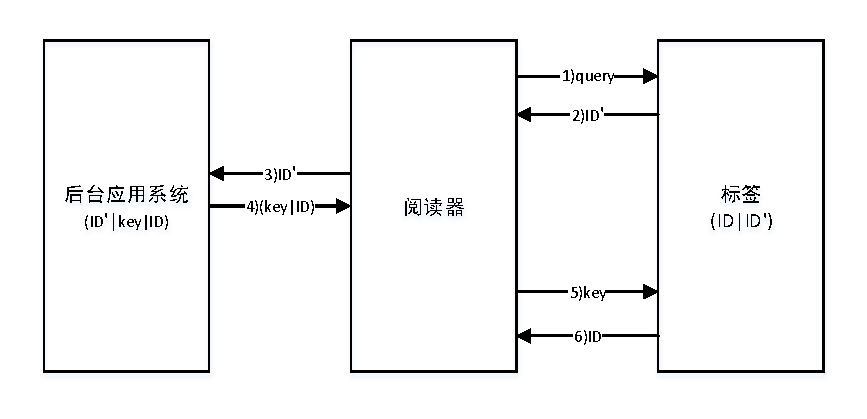
\includegraphics[width=\textwidth]{chap3/hashLock.pdf}
	\caption{Hash-Lock协议图示}\label{fig:Hash-Lock协议图示}
\end{figure}

1)当阅读器的识别范围内有电子标签进入时,阅读器向其发送query消息请求认证。

2)电子标签利用Hash函数对ID进行处理得到ID'发送给阅读器。

3)阅读器收到ID'后再发送给后台应用系统。

4)后台应用系统收到ID'后搜索所有标签,并计算对应的hash(ID)看是否与ID'相同,如果有就将ID与key发送给阅读器。

5)阅读器收到ID与key后保留ID,然后将key发送给标签。

6)标签收到key后,计算hash(key)看是否与ID相同,若相同则将ID发送给阅读器

7)阅读器将标签与后台应用系统发来的两个ID对比,如果相同则验证成功

\[\]

随机化Hash-Lock协议原理如图\ref{fig:随机化Hash-Lock协议图示}所示。

\begin{figure}[!htp]
	\centering
	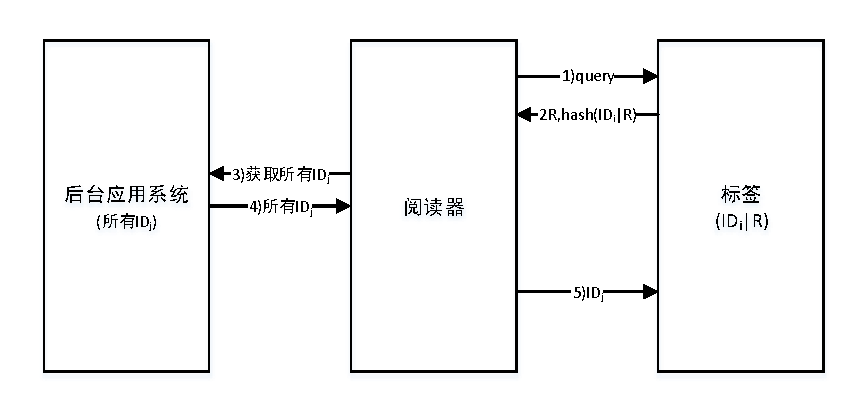
\includegraphics[width=\textwidth]{chap3/randomHashLock.pdf}
	\caption{随机化Hash-Lock协议图示}\label{fig:随机化Hash-Lock协议图示}
\end{figure}

1)当阅读器的识别范围内有电子标签进入时,阅读器向其发送query消息请求认证。

2)电子标签产生一个随机数R,然后利用Hash函数对ID及R的串接进行处理得到hash($ID_{i}$, R)发送给阅读器。

3)阅读器请求后台应用系统获取所有$ID_{j}$。

4)后台应用系统将所有$ID_{j}$发送给阅读器。

5)阅读器计算所有hash($ID_{j}$, R)看是否有$ID_{j}$能产生与hash($ID_{i}$, R)相同的结果,若有则将$ID_{j}$发送给标签。

6)标签收到$ID_{j}$后,看是否与与自身的$ID_{i}$相同,若相同则验证成功

\[\]

Hash链协议原理如图\ref{fig:Hash链协议图示}所示。

\begin{figure}[!htp]
	\centering
	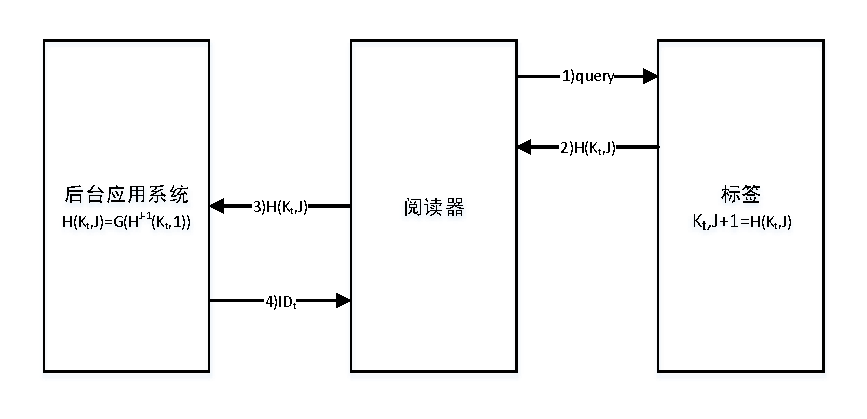
\includegraphics[width=\textwidth]{chap3/hashChain.pdf}
	\caption{Hash链协议图示}\label{fig:Hash链协议图示}
\end{figure}

1)当阅读器的识别范围内有电子标签进入时,阅读器向其发送query消息请求认证。

2)电子标签利用Hash函数加密密钥K$_{t}$,J(即H(K$_{t}$,J))发送给阅读器,同时更新当前的密码值K$_{t}$,J+1=H(K$_{t}$,J)。

3)阅读器收到电子标签发送来的H(K$_{t}$,J)继而转发给后台应用系统。

4)后台应用系统查找数据库搜索存储的所有标签,计算是否有某个标签的ID$_{t}$使得H(K$_{t}$,J)=G(H$^{J-1}$(K$_{t}$,1)),若有,认证通过,并把ID$_{t}$发送给电子标签。否则认证失败。

\[\]

基于Hash的ID变化协议原理如图\ref{fig:基于Hash的ID变化协议图示}所示。

\begin{figure}[!htp]
	\centering
	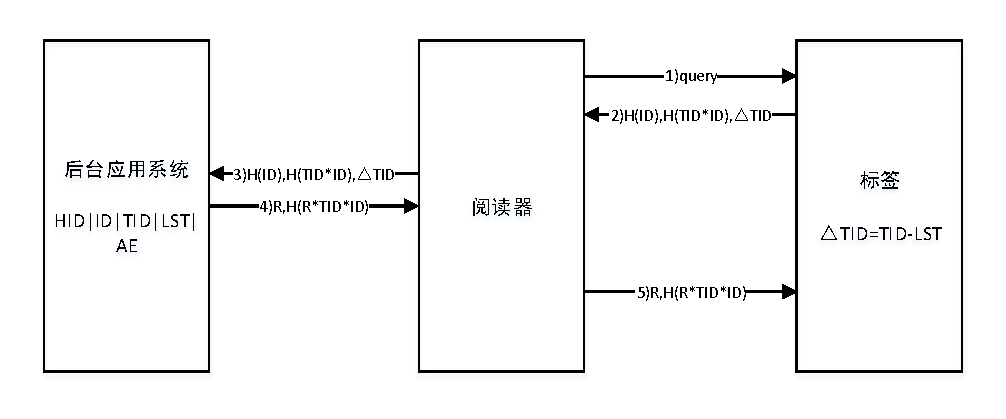
\includegraphics[width=\textwidth]{chap3/IDChangeHashChain.pdf}
	\caption{基于Hash的ID变化协议图示}\label{fig:基于Hash的ID变化协议图示}
\end{figure}

1)当阅读器的识别范围内有电子标签进入时,阅读器向其发送query消息请求认证。

2)电子标签将回话号加一,然后将H(ID),H(TID*ID),△TID发送给阅读器。

3)阅读器收到电子标签发送来的H(ID),H(TID*ID),△TID继而转发给后台应用系统。

4)后台应用系统还原出ID与TID*ID,与记录的数据比较,如果匹配上,产生随机数R,然后将R,H(R*TID*ID)发送给阅读器,然后同时更新TID、LST并将ID更新为ID异或R。

5)阅读器收到后再发给标签,标签收到后验证,如果通过则更新自己的ID和LST。

\[\]

David的数字图书馆RFID协议原理如图\ref{fig:David的数字图书馆RFID协议图示}所示。

\begin{figure}[!htp]
	\centering
	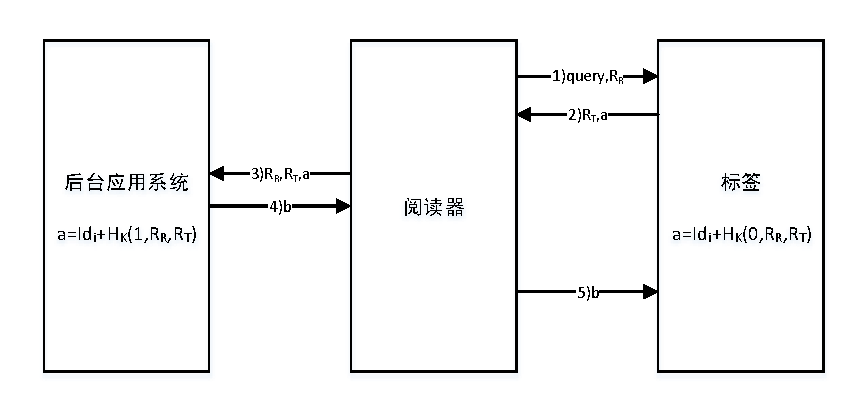
\includegraphics[width=\textwidth]{chap3/david.pdf}
	\caption{David的数字图书馆RFID协议图示}\label{fig:David的数字图书馆RFID协议图示}
\end{figure}

1)当阅读器的识别范围内有电子标签进入时,阅读器生成随机数$R_{R}$与query消息一起发送给标签请求认证。

2)电子标签产生随机数$R_{T}$,然后计算a=$ID_{i}+H_{k}(0,R_{R},R_{T})$并与$R_{T}$一起发送给阅读器。

3)阅读器收到的数据转发给后台应用系统。

4)后台应用系统比较所有标签看是否存在$ID_{j}$满足$ID_{j}=a+H_{k}(0,R_{R},R_{T})$,若有则认证通过,计算b=$ID_{i}+H_{k}(1,R_{R},R_{T})$并发送给阅读器。

5)阅读器收到后再发给标签,标签收到后验证是否满足ID=$b+ID_{i}+H_{k}(1,R_{R},R_{T})$,如果满足则认证成功。

\[\]

分布式RFID询问-应答认证协议原理如图\ref{fig:分布式RFID询问-应答认证协议图示}所示。

\begin{figure}[!htp]
	\centering
	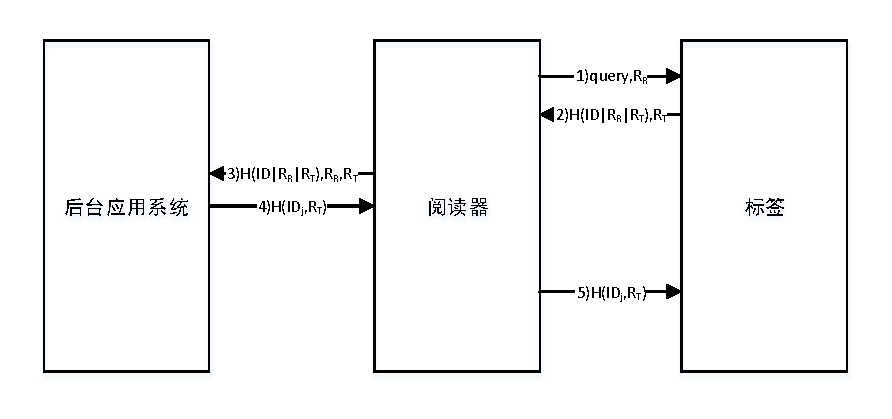
\includegraphics[width=\textwidth]{chap3/queryResponse.pdf}
	\caption{分布式RFID询问-应答认证协议图示}\label{fig:分布式RFID询问-应答认证协议图示}
\end{figure}

1)当阅读器的识别范围内有电子标签进入时,阅读器生成随机数$R_{R}$与query消息一起发送给标签请求认证。

2)电子标签产生随机数$R_{T}$,然后计算$H(ID||R_{R}||R_{T})$并与$R_{T}$一起发送给阅读器。

3)阅读器将收到的数据与$R_{R}$一起发给后台应用系统。

4)后台应用系统比较所有标签看是否存在$ID_{j}$满足$H(ID_{j}||R_{R}||R_{T})=H(ID||R_{R}||R_{T})$,若有则认证通过,计算$H(ID_{j}||R_{T})$并发送给阅读器。

5)阅读器收到后再发给标签,标签收到后验证是否满足$H(ID_{j}||R_{T})=H(ID||R_{T})$,如果满足则认证成功。

\[\]

LCAP协议原理如图\ref{fig:LCAP协议图示}所示。

\begin{figure}[!htp]
	\centering
	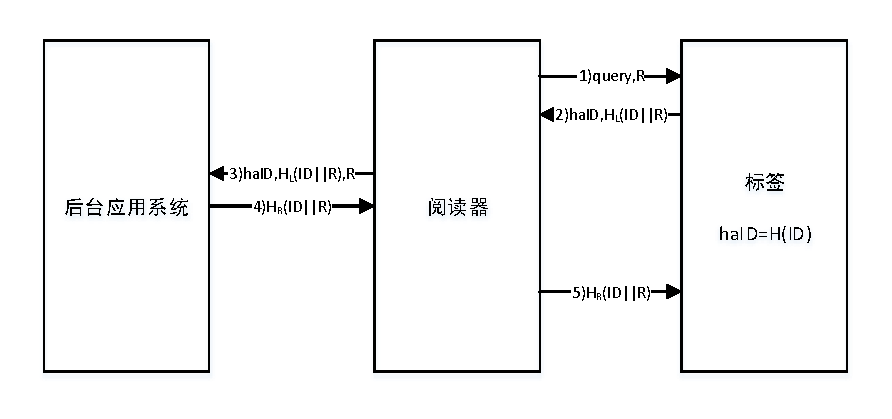
\includegraphics[width=\textwidth]{chap3/LCAP.pdf}
	\caption{LCAP协议图示}\label{fig:LCAP协议图示}
\end{figure}

1)当阅读器的识别范围内有电子标签进入时,阅读器生成随机数R与query消息一起发送给标签请求认证。

2)电子标签计算haID=H(ID)与H(ID||R)的左半部分即$H_{L}(ID||R)$一起发送给阅读器。

3)阅读器将收到的数据与R一起发给后台应用系统。

4)后台应用系统检查储存的haID是否与发来的一致,若一致,则利用hash函数计算R与haID得到$H_{R}(ID||R)$,同时更新haID为H(ID+R),更新ID为ID+R,并设置TD为H(ID+R),然后将$H_{R}(ID||R)$发送给阅读器。

5)阅读器收到后再发给标签,标签收到后验证有效性,如果成功则认证成功。

\[\]

根据网上资料\parencite{射频技术(RFID)的安全协议},这些基本的RFID协议的安全性如表\ref{tab:基本的RFID安全协议安全性分析}所示、性能如如表\ref{tab:基本的RFID安全协议性能分析}所示。

\begin{table}[!hbp]
	\newcommand{\tabincell}[2]{\begin{tabular}{@{}#1@{}}#2\end{tabular}} 
	\centering
	\caption{基本的RFID安全协议安全性分析}\label{tab:基本的RFID安全协议安全性分析}
	\begin{tabular}{|c|c|c|c|c|c|c|}
		\hline
		\hline
		安全协议 & \tabincell{c}{防窃听 \\ 攻击} & \tabincell{c}{防推理 \\ 攻击} & \tabincell{c}{防拒绝 \\ 服务攻击} & \tabincell{c}{防重放 \\ 攻击} & \tabincell{c}{防欺骗 \\ 攻击} & \tabincell{c}{防位置 \\ 追踪} \\
		\hline
		\tabincell{c}{Hash-Lock \\ 协议} & ${\texttimes}$ & ${\texttimes}$ & ${\surd}$ & ${\texttimes}$ & ${\texttimes}$ & ${\texttimes}$ \\
		\hline
		\tabincell{c}{随机化的 \\ Hash-Lock \\ 协议} & ${\surd}$ & ${\surd}$ & ${\texttimes}$ & ${\texttimes}$ & ${\texttimes}$ & ${\surd}$\\
		\hline
		\tabincell{c}{Hash链协议} & ${\surd}$ & ${\surd}$ & ${\texttimes}$ & ${\texttimes}$ & ${\texttimes}$ & ${\surd}$\\
		\hline
		\tabincell{c}{基于Hash的 \\ ID变化协议} & ${\surd}$ & ${\surd}$ & ${\texttimes}$ & ${\surd}$ & ${\texttimes}$ & ${\surd}$\\
		\hline
		\tabincell{c}{David的 \\ 数字图书馆 \\ RFID协议} & ${\surd}$ & ${\surd}$ & ${\texttimes}$ & ${\surd}$ & ${\surd}$ & ${\surd}$\\
		\hline
		\tabincell{c}{分布式RFID \\ 询问-应答 \\ 认证协议} & ${\surd}$ & ${\surd}$ & ${\texttimes}$ & ${\surd}$ & ${\surd}$ & ${\surd}$\\
		\hline
		LCAP & ${\surd}$ & ${\surd}$ & ${\texttimes}$ & ${\surd}$ & ${\surd}$ & ${\surd}$\\
		\hline
	\end{tabular}
\end{table}

\begin{table}[!hbp]
	\newcommand{\tabincell}[2]{\begin{tabular}{@{}#1@{}}#2\end{tabular}} 
	\centering
	\caption{基本的RFID安全协议性能分析}\label{tab:基本的RFID安全协议性能分析}
	\begin{tabular}{|c|c|c|c|c|c|c|}
		\hline
		\hline
		& \multicolumn{3}{c|}{计算时间} & \multicolumn{3}{c|}{存储容量} \\
		\cline{2-4}
		\cline{5-7}
		\hline
		安全协议 & 标签 & 阅读器 & 后台应用系统 & 标签 & 阅读器 & 后台应用系统\\
		\hline
		\tabincell{c}{Hash-Lock \\ 协议} & 1T$_{H}$ & - & - & 2L & - & 3nL\\
		\hline
		\tabincell{c}{随机化的 \\ Hash-Lock \\ 协议} & 1T$_{R}$,1T$_{H}$ & nT$_{H}$ & - & 1L & - & nL\\
		\hline
		\tabincell{c}{Hash链协议} & 2T$_{H}$ & - & 2nT$_{H}$ & 1L & - & 2nL\\
		\hline
		\tabincell{c}{基于Hash的 \\ ID变化协议} & 3T$_{H}$ & - & 1T$_{R}$,3T$_{H}$,2T$_{XOR}$ & 3L & - & 10nL\\
		\hline
		\tabincell{c}{David的 \\ 数字图书馆 \\ RFID协议} & 2T$_{XOR}$,1T$_{R}$ & 1T$_{R}$ & 2nT$_{XOR}$ & 2L & - & 2nL\\
		\hline
		\tabincell{c}{分布式RFID \\ 询问-应答 \\ 认证协议} & 1T$_{R}$,2T$_{H}$ & 1T$_{R}$ & (n+1)T$_{H}$ & 1L & - & nL\\
		\hline
		LCAP & 1T$_{R}$,1T$_{H}$ & - & 1T$_{H}$ & 2L & 1L & 1L\\
		\hline
	\end{tabular}
\end{table}

通过这些基本的RFID安全协议的安全性和性能对比,以及协议本身的实现方法,最终本文中将采用Hash链协议为基础协议,在此之上改造为使用Trivium算法。

选择Hash链协议的原因首先在于它每次都使用Hash函数更新发送给阅读器的信息,这点可以类比到Trivium算法每轮产生一个密钥上,还有就是在标签和后台应用系统之间共享了一个初始密钥K$_{t}$,1,这点可以类比到Trivium算法的密钥和初始向量,因此Hash链协议可以简单地把Hash函数替换成Trivium算法来加以实现。

\subsubsection{Trivium版RFID协议}

根据上节介绍的使用Trivium算法代替Hash链的RFID协议实现思路,尚存两个问题,第一个问题是具体到贵重物品追踪中,具体的硬件分配及所在位置,另一个问题是Trivium算法中密钥K、初始向量IV如何选择。

首先是硬件的问题,RFID协议涉及到三个硬件,分别是:后台应用系统、阅读器、标签,其中阅读器和标签的位置在之前已经提过,分别是在车内和物品上,那么问题就在于后台应用系统应该放在哪,一种选择是也放在车里,另一种自然是放在远程的数据中心。其实,只要看一下应用场景就可以知道是选择第一种。首要原因是使用RFID标签的目的是为了确定是否车内每一样物品都仍处于在车内的状态,这就要求需要阅读器周期性地扫描标签,并借由多个阅读器的定位确定标签的位置范围以确认标签是否在车内,因此这些阅读器本身需要一个统和的设施管理,于是后台应用系统就可以担任这个工作,每次认证通过后,阅读器再将与标签的距离信息发送给后台应用系统,然后后台应用系统根据所有阅读器对同一标签的距离计算出标签所在位置确认是否在车内。另一个原因是如果把后台应用系统放在远程,那还要考虑远程通信的方法,一种是随车辆的GPS信息一起发送,另一种是通过网络。但是随车辆的GPS信息发送的话,就要求GPS设备的厂商提供的开发接口能够实现发送用户自定义消息的功能,这点基本而言就已经不可能了,何况即使发出去,也没法接收。而通过网络的话,会有信号状态和延时问题。首先是延时,既然是远程通信那肯定要建立连接,而建立连接本身就会消耗很多时间,其次网络传输会有丢包问题,不断地超时重发,极可能到下一个检测周期,上一个检测周期的数据还没发出去,这时候就会产生误报发生物品丢失的情况。关键还在于信号问题,起码现在,在隧道这种地方信号都是很差的,而运输业走隧道的可能性还是很高的,不可能因为为了防止信号不好就让运输车绕远路,这反而是一种本末倒置,更何况现在也不是世界各地每个地方都有无线网覆盖,从起点到终点要选择一条全程被无线网覆盖的路线也不是一件轻松的事。所以综合考虑,还是直接将后台应用系统也放在车内比较合适。

其次是Trivium算法中密钥K(key)、初始向量IV的选择问题。一般而言,流密码中用来确定生成序列的函数的参数被称为Key,而这个序列用来作为初始值启动的=记成向量的形式就叫初始向量IV,所以通常而言,Key是保密的且不怎么变化,而IV有时保密有时公开,且变化频繁,每次加密都可以更换。虽然在Trivium算法中K和IV显得非常平等,仅仅是所处位置不同,但仍可以基于上述原则对K和IV进行选择。由于标签的ID通常是保密的,且不是经常更换或者无法更换的,另外每一次运输过程,运输公司通常会有内部运输号,因此可以将标签的ID即$ID_{T}$作为K。至于IV,由于每次加密过程IV都是更换的,所以可以让阅读器每次发出请求时附带一个随机数r,将这个随机数作为IV使用,而运输号$ID_{V}$可以用作标签验证阅读器。

改造后的协议如图\ref{fig:Trivium版RFID协议图示}所示。

\begin{figure}[!htp]
	\centering
	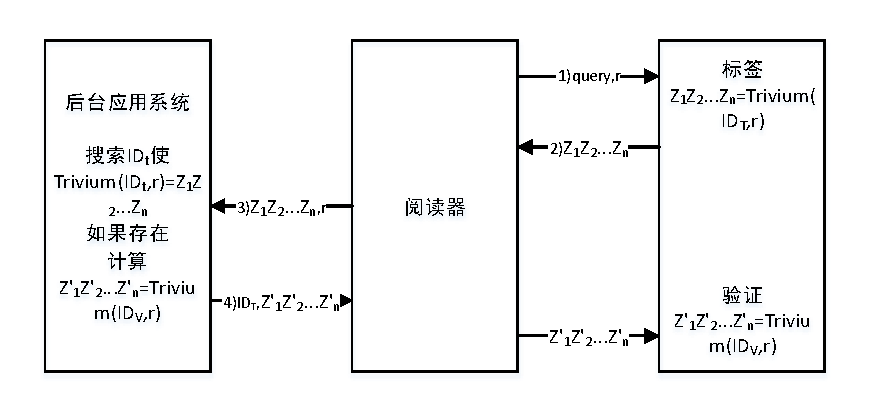
\includegraphics[width=\textwidth]{chap3/triviumChain.pdf}
	\caption{Trivium版RFID协议图示}\label{fig:Trivium版RFID协议图示}
\end{figure}

1)当阅读器的识别范围内有电子标签进入时,阅读器向其发送query消息及随机数r请求认证。

2)电子标签根据密钥和初始向量运行n轮Trivium,得到n位长的密钥流Z$_{1}$ Z$_{2}$... Z$_{n}$,将其发给阅读器。

3)阅读器收到电子标签发送来的Z$_{1}$ Z$_{2}$... Z$_{n}$继而和随机数r一起转发给后台应用系统。

4)后台应用系统查找数据库搜索存储的所有标签,计算是否有某个标签的$ID_{T}$作为K,r作为IV,运行n轮Trivium算法得到密钥流等于$Z_{1}$ $Z_{2}$... $Z_{n}$,若有,认证通过,然后后台应用系统以运输号$ID_{V}$作为K,r作为IV,运行n轮Trivium算法得到密钥流$Z'_{1}$ $Z'_{2}$... $Z'_{n}$并把$ID_{T}$与$Z'_{1}$ $Z'_{2}$... $Z'_{n}$发送给阅读器,阅读器收到后再将$Z'_{1}$ $Z'_{2}$... $Z'_{n}$发送给标签,标签以运输号$ID_{V}$作为K,r作为IV,运行n轮Trivium算法看得到的n位密钥流是否与$Z'_{1}$ $Z'_{2}$... $Z'_{n}$相等。否则认证失败。

\subsubsection{硬件设计}

综合之前的设计,贵重物品追踪的硬件设计如图\ref{fig:贵重物品追踪的硬件设计}所示。

\begin{figure}[!htp]
	\centering
	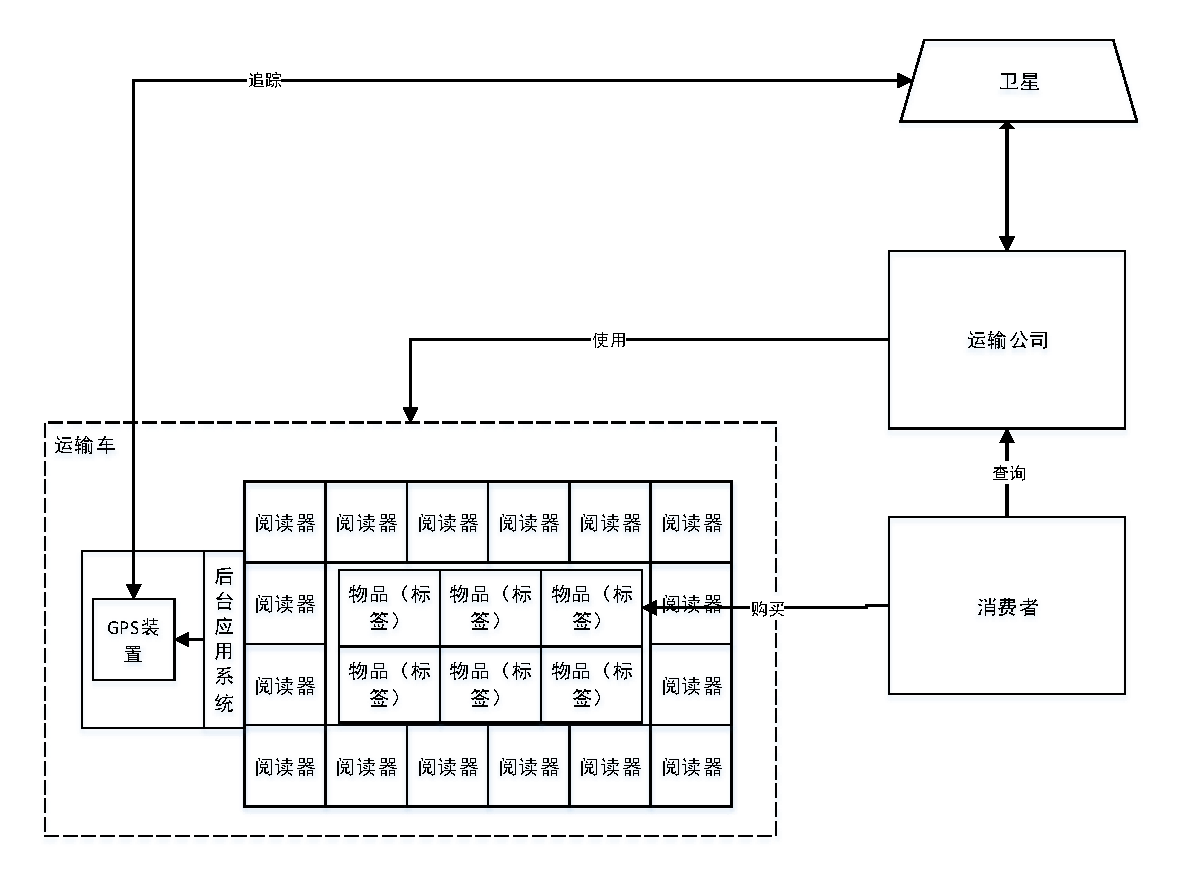
\includegraphics[width=\textwidth]{chap3/design.pdf}
	\caption{贵重物品追踪的硬件设计}\label{fig:贵重物品追踪的硬件设计}
\end{figure}

1)消费者购买物品

2)运输公司对每件物品贴上RFID标签,并为每个标签录入本次运输号

3)运输公司向后台应用系统录入本次所有标签ID及本次运输号

4)后台应用系统周期性控制阅读器检测所有标签位置

5)运输公司通过GPS定位追踪运输车

6)消费者可以向运输公司查询当前所购物品位置

\subsection{安全性分析}

\subsubsection{Trivium版RFID协议防欺骗攻击}

攻击者首先假扮成合法的阅读器向标签发出请求query并附带随机数r,标签收到请求后,运行Trivium算法对随机数r进行加密得到C,返回给阅读器。下一次认证会话时真正的合法阅读器向标签发出请求query并附带随机数r’,攻击者假扮成标签返回C。但由于每次认证会话中阅读器都会产生新的随机数,即r≠r’,所以攻击者无法假扮标签进行欺骗攻击。

\subsubsection{Trivium版RFID协议防重放攻击}

合法阅读器向标签发出请求query并附带随机数r,标签返回的Z$_{1}$ Z$_{2}$... Z$_{n}$被攻击者截取,下一次认证会话时合法阅读器向标签发出请求query并附带随机数r’,攻击者假扮标签返回Z$_{1}$ Z$_{2}$... Z$_{n}$。但由于每次认证会话中阅读器都会产生新的随机数,即r≠r’,而攻击者想返回对应的密钥流需要知道标签的ID和运输号,因此攻击者无法假扮标签进行重放攻击。

\subsubsection{Trivium版RFID协议的Ban逻辑分析}

上面已经分别分析了防欺骗攻击和防重放攻击,下面以Ban逻辑进行安全分析,以得到更准确的结论。

(1)首先建立基本模型,在本基本模型中,将后台应用系统与阅读器合并作为一个主体A,将标签作为主体B:

1)A $\rightarrow$ B: A向B发送认证请求{query, $N_{a}$}

2)B $\rightarrow$ A: B向A发送${ID_{T}, N_{a}}_{Trivium}$作为应答,其中Trivium为A与B之间共享的的秘密

3)A: A收到${ID_{T}, N_{a}}_{Trivium}$后对B进行身份认证查看其合法性,如果认证通过则转到第(4)步,否则认证失败停止

4)A $\rightarrow$ B: A向B发送${ID_{V}, N_{a}}_{Trivium}$,其中Trivium为A与B之间共享的的秘密

5)B: B收到${ID_{V}, N_{a}}_{Trivium}$后对A进行身份认证查看其合法性,如果认证失败则停止,否则认证通过

\[\]

(2)Ban理想化模型:

B $\rightarrow$ A: ${ID_{T}, N_{a}}_{Trivium}$

A $\rightarrow$ B: ${ID_{V}, N_{a}}_{Trivium}$

\[\]

(3)假定:

A believes A $\xleftrightarrow{Trivium}$ B \\
B believes A $\xleftrightarrow{Trivium}$ B \\
A believes fresh($N_{a}$) \\
B believes fresh($N_{a}$) \\
A believes (B controls A $\xleftrightarrow{ID_{T}}$ B) \\
B believes (A controls A $\xleftrightarrow{ID_{V}}$ B) \\

\[\]

(4)推理

A sees ${ID_{T}, N_{a}}_{Trivium}$ \\
由A believes A $\xleftrightarrow{Trivium}$ B 及 P sees(X, Y) $\rightarrow$ P sees(X) 及 P believes Q $\xleftrightarrow{K}$ P, P sees ${X}_{K}$ $\rightarrow$ P believes Q said X \\
可推出A believes B said {$ID_{T}, N_{a}$} 及 A believes B said $ID_{T}$\\
由A believes fresh($N_{a}$) 及 P believes fresh(X) $\rightarrow$ P believes fresh(X,Y) \\
可推出A believes fresh($ID_{T}$)\\
由P believes fresh(X), P believes Q said X $\rightarrow$ P believes Q believes X \\
可推出A believes B believes $ID_{T}$ \\
同理可推出B believes A believes $ID_{V}$

(5)结论

通过Ban逻辑的形式化证明,推出A believes B believes $ID_{T}$ 和B believes A believes $ID_{V}$,由此证明本Trivium版RFID协议可以实现标签与阅读器的双向认证。



\subsubsection{物品安全}

如之前所述,物品安全由GPS装置与RFID标签两部分共同保证。

对整辆运输车被劫取的保护:如果整辆运输车被劫取,那么运输公司在对运输车辆的追踪中会发现车辆偏离原始的行进路线。如果犯罪分子发现GPS装置并试图移除,那么运输公司可以监测到GPS被移除的现象并定位到最后位置。

对货物的偶然丢失保护:如果在运输过程中,由于车辆晃动等偶然原因造成物品掉落出运输车,那么在后台应用系统周期性控制阅读器检测所有标签位置过程中,会发现标签数量不符合并能定位哪些标签消失,此时后台应用系统向GPS装置发送消息,由GPS装置经由卫星向运输公司发出消息通知哪个标签于何处消失,运输公司根据标签ID及运输车辆的运输号查询到是什么物品丢失,并通过工作人员在丢失位置附近搜索。

对货物的人为丢失保护:如果在运输过程中发生由人为引起的物品离开运输车,那么同理运输公司可以定位是在何处丢失了什么物品。如果有人试图假冒标签对阅读器进行欺骗或重复以在将物品移除运输车后营造物品仍存在的假象,那么根据之前对Trivium版RFID协议的安全性分析,这是无法做到的。然而如果发生仅取走货物,而将货物对应的标签留在运输车内,那么此时便无法被探知,并且也无法定位货物是在何处被偷。

对货物位置的隐私保护:货物位置在理论上应该仅有运输公司及消费者本人可以获知。对于同过网络查询货物位置的一系列通信保护和身份认证系统,现在已经有许多成熟的架构可以实现,对此,本设计不考虑这方面的额外安全保护设计。但是货物的位置信息仍存在物理手段的窃取可能,即进入运输车仅检查货物信息并不取走货物,此时无法通过RFID标签系统探知这种行为,但货物的位置信息被得知。对于这种问题,存在一种解决方案,将货物封入运输包装时,将RFID标签贴在封口的里侧,即从外侧无法接触到RFID标签,而要打开运输包装需要折断RFID标签,这就包装在送到消费者之前如果有人试图确认货物内部,那么就会造成该货物对应的RFID标签折断,进而触发货物丢失的警报。但是这么做有成本问题,因为如果每次都要折断RFID标签, 那么标签就从可重复利用型硬件转为一次性消耗型硬件,那么此时无论标签是由运输公司承担还是消费者个人承担,最终这一成本都会转化为消费者所购物品的价格上升,并且之前也提到本设计中使用的RFID标签为有源标签,所以成本很高,所以本设计并不采用这种防范措施,而只能寄希望于运输人员的安全意识以及自觉或者是未来有源标签的成本下降。

\section{其他应用}

\subsection{加密手机}

加密手机的大致构思是加密手机可以在加密模式和非加密模式之间切换,当切换到加密模式后,可以和另一部处于加密模式的手机进行密钥协商,然后进行加密通信,其他不支持加密的手机无法和它通信,这种手机非常适合商务人士或者军队使用。实现的话可以考虑在手机内加装一个SoC模块。

具体实现中的问题主要集中在如何协商密钥和如何加密通信两块。加密通信这块,在分析Trivium算法在物联网中应用的优势时已经提到,Trivium算法的高效性非常适合手机通话这样对实时性有高要求的场景,另外手机通话通常连续通话时间不会特别漫长,最多以小时计量,而根据之前对Trivium算法安全性的分析,现今的攻击手段所耗的时间,即便是对削弱的Trivium算法也未必能在通话时间内攻破,所以安全性很有保证。而协商密钥这块,比较经典的基于证书的密钥协商协议有经典Diffie-Hellman协议、MTI协议族、MQV协议。但是手机号现在没有证书这一说,所以伪基站可以仿冒别人发短信,因此也谈不上使用基于证书的密钥协商协议。而对其他不需要证书的密钥协商协议以及把证书不是绑定在手机号上而是其他位置的研究由于时间原因还未研究,因此这一想法暂时被搁置,有待以后再研究。

\subsection{无钥匙取车}

出行是日常生活的重要组成部分,因此现在很多公司都瞄准这一块,把互联网思维带到这个领域,由此诞生出了打车软件、租车软件等等。无钥匙取车正是属于租车软件中的一环,以pp租车为例,pp租车是让车主装一个pp租车提供的装置,然后要将车出租时,将车停到指定位置后把钥匙留在车内,然后用提供的装置将车门锁上,租车人要租车时,就到指定位置,使用手机上的app将装置解锁,进入车内使用钥匙启动车辆。

现有的无钥匙取车方案有两种:第一种就是上述提到的,通过手机中的app扫描二维码对车门进行解锁,然后使用预先放在车内的钥匙,这种方案在P2P租车中普遍应用;另一种被称为PKES系统,车主在打开车门和启动汽车的时候并不需要拿出钥匙按一下按钮或者插进锁中而只需要揣在口袋里,由车辆进行扫描,这种方案在一些高档汽车中有出现。

虽然上面两种方案都可以把Trivium算法用于身份认证套进去,但因为在无钥匙取车这个场景下并没有很高的实时性要求,想反,比起身份认证更应该关注物理安全,比如钥匙放车内,要是有人打破车窗拿了钥匙开走车怎么办,所以尚未有一定要使用Trivium算法的必要性,因此这个场景只能说也能用Trivium算法但并非侧重点,因此该场景未进一步研究。

\section{本章小结}

本章首先介绍了Trivium算法在物联网中使用的优势,并粗略介绍了目前对Trivium算法的攻击进展情况。接着基于Trivium算法的优势,本章介绍了在贵重物品追踪中使用Trivium算法的设计,包括了从硬件部署到协议的设计,然后分析了这种设计下是否具有数据传输的私密性以及物品安全的保障。最后本章介绍了其他能够使用Trivium算法的应用场景的背景和大致思路。

%%==================================================
%% conclusion.tex for SJTUThesis
%% Encoding: UTF-8
%%==================================================

\begin{summary}

  

\end{summary}


\appendix	% 使用英文字母对附录编号,重新定义附录中的公式、图图表编号样式
\renewcommand\theequation{\Alph{chapter}--\arabic{equation}}	
\renewcommand\thefigure{\Alph{chapter}--\arabic{figure}}
\renewcommand\thetable{\Alph{chapter}--\arabic{table}}
\renewcommand\thealgorithm{\Alph{chapter}--\arabic{algorithm}}

%% 附录内容,本科学位论文可以用翻译的文献替代。
% %%==================================================
%% Encoding: UTF-8
%%==================================================

\chapter{模板更新记录}
\label{chap:updatelog}

\textbf{2015年3月15日} v0.8发布,使用biber/biblatex组合替代 \BibTeX ,带来更强大稳定的参考文献处理能力;添加enumitem宏包增强列表环境控制能力;完善宏包文字描述。

\textbf{2015年2月15日} v0.7发布,增加盲审选项,调用外部工具插入扫描件。

\textbf{2015年2月14日} v0.6.5发布,修正一些小问题,缩减git仓库体积,仓库由sjtu-thesis-template-latex更名为SJTUThesis。

\textbf{2014年12月17日} v0.6发布,学士、硕士、博士学位论文模板合并在了一起。

\textbf{2013年5月26日} v0.5.3发布,更正subsubsection格式错误,这个错误导致如"1.1 小结"这样的标题没有被正确加粗。

\textbf{2012年12月27日} v0.5.2发布,更正拼写错误。在diss.tex加入ack.tex。

\textbf{2012年12月21日} v0.5.1发布,在 \LaTeX 命令和中文字符之间留了空格,在Makefile中增加release功能。

\textbf{2012年12月5日} v0.5发布,修改说明文件的措辞,更正Makefile文件,使用metalog宏包替换xltxtra宏包,使用mathtools宏包替换amsmath宏包,移除了所有CJKtilde(\verb+~+)符号。

\textbf{2012年5月30日} v0.4发布,包含交大学士、硕士、博士学位论文模板。模板在\href{https://github.com/weijianwen/sjtu-thesis-template-latex}{github}上管理和更新。

\textbf{2010年12月5日} v0.3a发布,移植到 \XeTeX/\LaTeX 上。

\textbf{2009年12月25日} v0.2a发布,模板由CASthesis改名为sjtumaster。在diss.tex中可以方便地改变正文字号、切换但双面打印。增加了不编号的一章“全文总结”。
添加了可伸缩符号(等号、箭头)的例子,增加了长标题换行的例子。

\textbf{2009年11月20日} v0.1c发布,增加了Linux下使用ctex宏包的注意事项、.bib条目的规范要求,
修正了ctexbook与listings共同使用时的断页错误。

\textbf{2009年11月13日} v0.1b发布,完善了模板使用说明,增加了定理环境、并列子图、三线表格的例子。

\textbf{2009年11月12日} 上海交通大学硕士学位论文 \LaTeX 模板发布,版本0.1a。


% %% app2.tex for SJTU Master Thesis
%% based on CASthesis
%% modified by wei.jianwen@gmail.com
%% version: 0.3a
%% Encoding: UTF-8
%% last update: Dec 5th, 2010
%%==================================================

\chapter{Maxwell Equations}

选择二维情况,有如下的偏振矢量:
\begin{subequations}
  \begin{eqnarray}
    {\bf E}&=&E_z(r,\theta)\hat{\bf z} \\
    {\bf H}&=&H_r(r,\theta))\hat{ \bf r}+H_\theta(r,\theta)\hat{\bm
      \theta}
  \end{eqnarray}
\end{subequations}
对上式求旋度:
\begin{subequations}
  \begin{eqnarray}
    \nabla\times{\bf E}&=&\frac{1}{r}\frac{\partial E_z}{\partial\theta}{\hat{\bf r}}-\frac{\partial E_z}{\partial r}{\hat{\bm\theta}}\\
    \nabla\times{\bf H}&=&\left[\frac{1}{r}\frac{\partial}{\partial
        r}(rH_\theta)-\frac{1}{r}\frac{\partial
        H_r}{\partial\theta}\right]{\hat{\bf z}}
  \end{eqnarray}
\end{subequations}
因为在柱坐标系下,$\overline{\overline\mu}$是对角的,所以Maxwell方程组中电场$\bf E$的旋度:
\begin{subequations}
  \begin{eqnarray}
    &&\nabla\times{\bf E}=\mathbf{i}\omega{\bf B} \\
    &&\frac{1}{r}\frac{\partial E_z}{\partial\theta}{\hat{\bf
        r}}-\frac{\partial E_z}{\partial
      r}{\hat{\bm\theta}}=\mathbf{i}\omega\mu_rH_r{\hat{\bf r}}+\mathbf{i}\omega\mu_\theta
    H_\theta{\hat{\bm\theta}}
  \end{eqnarray}
\end{subequations}
所以$\bf H$的各个分量可以写为:
\begin{subequations}
  \begin{eqnarray}
    H_r=\frac{1}{\mathbf{i}\omega\mu_r}\frac{1}{r}\frac{\partial
      E_z}{\partial\theta } \\
    H_\theta=-\frac{1}{\mathbf{i}\omega\mu_\theta}\frac{\partial E_z}{\partial r}
  \end{eqnarray}
\end{subequations}
同样地,在柱坐标系下,$\overline{\overline\epsilon}$是对角的,所以Maxwell方程组中磁场$\bf H$的旋度:
\begin{subequations}
  \begin{eqnarray}
    &&\nabla\times{\bf H}=-\mathbf{i}\omega{\bf D}\\
    &&\left[\frac{1}{r}\frac{\partial}{\partial
        r}(rH_\theta)-\frac{1}{r}\frac{\partial
        H_r}{\partial\theta}\right]{\hat{\bf
        z}}=-\mathbf{i}\omega{\overline{\overline\epsilon}}{\bf
      E}=-\mathbf{i}\omega\epsilon_zE_z{\hat{\bf z}} \\
    &&\frac{1}{r}\frac{\partial}{\partial
      r}(rH_\theta)-\frac{1}{r}\frac{\partial
      H_r}{\partial\theta}=-\mathbf{i}\omega\epsilon_zE_z
  \end{eqnarray}
\end{subequations}
由此我们可以得到关于$E_z$的波函数方程:
\begin{eqnarray}
  \frac{1}{\mu_\theta\epsilon_z}\frac{1}{r}\frac{\partial}{\partial r}
  \left(r\frac{\partial E_z}{\partial r}\right)+
  \frac{1}{\mu_r\epsilon_z}\frac{1}{r^2}\frac{\partial^2E_z}{\partial\theta^2}
  +\omega^2 E_z=0
\end{eqnarray}

% \chapter{从 \CJKLaTeX 转向 \XeTeX }
\label{chap:whydvipdfm}

我习惯把v0.2a使用dvipdfmx编译的硕士学位论文模板称为“ \CJKLaTeX 模板”,而这个使用 \XeTeX 引擎(xelatex程序)处理的模板则被称为“{\XeTeX/\LaTeX}模板”。
从 \CJKLaTeX 模板迁移到{\XeTeX\LaTeX}模板的好处有下:
\begin{enumerate}
\item[\large\smiley] 搭建 \XeTeX 环境比搭建 \CJKLaTeX 环境更容易;
\item[\large\smiley] 更简单的字体控制;
\item[\large\smiley] 完美支持PDF/EPS/PNG/JPG图片,不需要“bound box(.bb)”文件;
\item[\large\smiley] 支持OpenType字体的复杂字型变化功能;
\end{enumerate}

当然,这也是有代价的。由于 \XeTeX 比较新,在我看来,使用 \XeTeX 模板所必须付出的代价是:

\begin{enumerate}
\item[\large\frownie] 必须把你“古老的” \TeX 系统更新为较新的版本。TeXLive 2012和CTeX 2.9.2能够编译这份模板,而更早的版本则无能为力。
\item[\large\frownie] 需要花一些时间把你在老模板上的工作迁移到新模板上。
\end{enumerate}

第一条就看你如何取舍了,新系统通常意味着更好的兼容性,值得升级。而转换模板也不是什么特别困难的事情,可以这样完成:

\begin{enumerate}
\item 备份你要转换的源文件,以防你的工作成果丢失;
\item 将你原来的tex以及bib文件另存为UTF-8编码的文件。iconv、vim、emacs、UEdit等等工具都可以完成。WinEdt对文件编码识别功能很差(到了v6.0还是如此),不推荐作为字符编码转换工具;
\item 将diss.tex导言区中的内容替换为XeTeX模板diss.tex导言区的内容;
\item 将你对原先导言区的修改,小心翼翼地合并到新的导言区中;
\item 使用XeTeX模板中的GBT7714-2005NLang.bst替换原有的bst文件,新的bst文件只是将字符编码转换为UTF-8;
\item 删除bouding box文件;
\item 使用本文\ref{sec:process}介绍的方法,重新编译文档;
\end{enumerate}



\backmatter	% 文后无编号部分 

%% 参考资料
\printbibliography[heading=bibintoc]

%% 致谢、发表论文、申请专利、参与项目、简历
%% 用于盲审的论文需隐去致谢、发表论文、申请专利、参与的项目
\makeatletter
%%==================================================
%% thanks.tex for SJTU Master Thesis
%% based on CASthesis
%% modified by wei.jianwen@gmail.com
%% version: 0.3a
%% Encoding: UTF-8
%% last update: Dec 5th, 2010
%%==================================================

\begin{thanks}

首先感谢我的导师陈恭亮教授,在本次毕业设计中,陈老师除了在研究方面教导我们一步步学会如何针对一个密码系统进行研究,而且让我们学会做研究不能仅专注于理论上分析,如果设法将研究对象应用于一个实际应用场景中,那么在此分析研究过程中可能能收获更多。在此向陈老师表达最真挚的感谢。

另外这里还要感谢王健同学和张诗永学长。王健同学作为和我同样处于陈老师带领的毕业设计的学生,由于我们的研究内容有交集,因此有很多时候都是在与王健同学的探讨中激发出灵感或者发现需要改正的问题。张诗永学长作为我们的前辈,对我们研究的内容有深刻的理解和丰富的知识,在我们手足无措时经常是在张学长耐心的讲解下,我们才能明确下一步该怎么走比较好。在此对王健同学和张诗永学长表示万分感谢。

最后在此感激我的室友们和朋友们,他们在我四年的大学生活及论文的协作过程中不仅给予我学习上的鼓舞和帮助,更是在生活为人方面给了我很多帮助和启迪,虽然在此无法一一列举他们的名字,但在此请让我致以感谢。

\end{thanks}

\makeatother

\begin{bigabstract}
With the informatization of society, the Earth has become the global village and the contact between people is closer. Now the conception of the IoT(Internet of Things) rises and the Earth is ready to accept another revolution. Experimental products like smart furniture and car networking appear in the market. The media describes the future life which is full of IoT as beautiful as a painting. Though the IoT may make our life more convenient, it is irresponsible that the media only introduces the advantages of the Iot without mentioning the disadvantages at the meantime. We have seen how destructive it is when the secure incidents occur in the Internet though no doubt that the Internet has brought good change to our life. What we should learn is that everything has its good side and bad side. When we talk about the convenience the IoT may brought, we should not forget that the IoT may also be dangerous. For example, factories may stop producing, cars may become out of control, smart furniture may cause fire. So the security of the IoT should be paid attention to.

Another problem is that there isn’t an exact definition of the IoT even now. In 1999, MITAutoIDCenter gave the early definition of the IoT: using RFID/wireless communication technology to build an Internet of Things based on the Internet. In 2005, ITU formally gave the conception of the IoT and expanded its meaning. It pointed out that the IoT was the expansion of the Internet and four core technology to realize the IoT was RFID, sensor technology, nanotechnology and intelligent embedding technology. In 2009, EU published CERPIoTSRA which defined the IoT as indivisible part of the Internet and a dynamic global networking frame which had self- organized ability based on certain standard and communication protocols. Though there isn’t an exact definition of the IoT and there is no standard now, secure standard will no doubt be a must.

Nowadays, there are various research about the IoT because it is regarded as strategic developing aim. But most paper focuses on the developing direction or the frame of the IoT, and some just adapt the IoT to systems in other area while few research the possible security problems in the IoT. So it is meaningful to research the secure problems in the IoT.

Since various things with different chips within them will be connected to the IoT, encryption algorithm like RSA/AES may not be suitable because of the difference in computing ability of those chips. So a lightweight cryptographic algorithm is needed which could be used even in chips whose computing ability isn’t pretty strong. And Trivium is exactly a lightweight cryptographic algorithm, so it is possible that Trivium may be the cryptographic algorithm in the IoT in the future. 

Trivium is a hardware-based stream cipher algorithm, which is one of eSTREAM Project's final victorious algorithms. It is proposed by Christophe De Canniere and Bart Preneel. It gained great attention once it was published because of its simple and elegant design. It was designed to see if an algorithm could be simple without sacrificing its security, efficiency and flexibility. Trivium also declares that it is very secure. And until April 2015, several attacks are close to break Trivium. First an attack due to Michael Vielhaber broke a variant of Trivium where the number of initialization rounds was reduced to 576 in only 212.3 steps. Then other authors speculated that attacks which built on Michael Vielhaber’s could lead to a break for 1100 initialization rounds or even the original Trivium. Then the cube attack which need 268 steps to break a variant of Trivium where reducing the number of initialization rounds to 799. Another attack use around 289.5 steps (where each step is roughly the cost of a single trial in exhaustive search) to recover the internal state (and thus the key) of the full cipher. By using an equation-solving technique reduced variants of Trivium using the same design principles have been broken. Though these attacks are close to succeed in breaking Trivium, these attacks all have their own supposition. For example, some reduce the number of the initialization rounds in the origin Trivium, some suppose that they can control the plaintext, and some even suppose that they can control the internal states. It was these supposition that make their attacks break the variant Trivium and it was these supposition that make their attacks close to succeed in breaking the origin Trivium instead of succeeding in breaking the origin Trivium. For example, some suppose that they can control the plaintext, and it is possible in most situation, but in the IoT chips may only send the set message and thus make it more difficult control the plaintext. And we should notice that the best attack method until April 2015 was still brute force attack, so Trivium is still a secure algorithm, and we can use it in the IoT.

Trivium is still a new algorithm and there isn’t much research on Trivium, and most as mentioned above study the security of Trivium by trying to break it. But there is rarely research on Trivium itself like the structure of Trivium, what should be paid attention to when design the algorithm which is similar to the origin Trivium, not mentioning the application of Trivium. But we may learn more about Trivium when trying to adapt it to a real application environment. When we try to adapt Trivium to a real-world scenario, we will have several mark like the efficiency and security needed in the IoT. And when we try to improve Trivium to reach these marks, we may learn more about Trivium. So it is meaningful to study how to adapt Trivium to a real-world scenario.

In this paper, we study Trivium in two ways. In one way, we study the Trivium algorithm itself like what the structure Trivium has or the period of Trivium. While in the other way, we suppose that we use Trivium in a real-world scenario and see if Trivium is suitable for the scenario. If Trivium doesn’t work well in this scenario, we try to improve it.

In the first chapter, we simply introduce the Trivium algorithm and the development of the IoT. We will see the truth that from 1999 till now, though the IoT has developed so long, there is not even a definitely definition. We will introduce 3 different definition in different time.

In the second chapter, we will introduce the Trivium algorithm in detail. First, we introduce the traditional Trivium. We will introduce how to use Trivium to generate key stream, how to initialize the internal states of Trivium and how to realize Trivium by hardware. Then we will analyze the structure of Trivium. We will analyze the state-transition matrix of Trivium. And we will parameterize Trivium, which we call the Trivium type algorithm. Finally, we will study the period of the linear part of Trivium, and then the nonlinear part. We will try to construct some internal states which will lead to the appearance of minor cycle in Trivium. We try to construct these internal states so that when we try to use Trivium, we can avoid using these internal states to keep Trivium safe. And then, we expend the way we create minor cycle in Trivium to the Trivium Type algorithm especially the period 3. And we prove that the way we create period 3 is pervasive in all Trivium type algorithm.

In the third chapter, we will try to suppose a real-world scenario where we will use Trivium. First, we will analyze why we should use Trivium in the IoT like what are the advantages if we use Trivium in the IoT. We will judge it by analyzing the efficiency and secure of Trivium. When judging the efficiency of Trivium, we will give an approximate logic gate number of Trivium, and give an approximate contrast between the encryption speed of Trivium and AES. When judging the secure of Trivium, we will give some current attacks on Trivium such as Cube Attack, Floating Fault Attack, Differential Fault Attack and so on. But we will see that until now the best attack on Trivium is still brute force attack and that’s why we think Trivium is secure. Then we will try to adapt Trivium in tracking valuables. We will introduce the background of tracking valuables first, and then the design. How to locate the valuables will be the first part of the design. Then several RFID protocols such as Hash-Lock Protocol, Random Hash-Lock Protocol, Hash-Chain Protocol, ID change Protocol based on Hash, David's Digital Library Protocol and Distributed RFID Request and Response Protocol will be introduced and they will be analyzed to see their efficiency and secure and then choose one to change to the Trivium type. The design of Trivium type RFID protocol will be the third part of the total design. We design the Trivium Type RFID protocol based on Hash-Chain Protocol which is easier to change to Trivium among other basic RFID protocols. After we give the design of Trivium type RFID protocol, we will analyze its security. We will analyze whether the new protocol could work against the cheat attack and the relay attack. And we will use ban logic to analyze whether it could provide a safe mutual authentication formally. And the design of hardware will be the final part where we will show the frame diagram of the whole design. Then we will analyze whether the design is reasonable which means we will discuss whether the privacy of communication is assured and whether the valuables can be kept safely. Finally, we will raise some other scenario where Trivium may also be used and make the conclusion of this chapter.

In the last chapter, we will make the conclusion. We will summarize what we achieve from this research and what’s the research directions in the future.

\end{bigabstract}

\end{document}
